\documentclass[a4j]{jsbook}
\usepackage[top=20truemm,bottom=25truemm,left=25truemm,right=25truemm]{geometry}
\usepackage{amsmath}
\usepackage{bm}
\usepackage{float}
\usepackage{fancyvrb}
%\usepackage{moreverb}
\usepackage{listings,jlisting}
%\usepackage{color}
\usepackage{comment}
\usepackage[dvipdfmx]{graphicx,psfrag,color}
%\usepackage{graphicx}
\usepackage{subfig}

\lstset{%
  language={Fortran},
  basicstyle={\small},%
  basicstyle=\ttfamily,
  identifierstyle={\small},%
  commentstyle={\small\color[rgb]{0,0.5,0}},%
  keywordstyle={\small\bfseries\color[rgb]{0,0,1}},%
  ndkeywordstyle={\small},%
  stringstyle={\small\ttfamily\color[rgb]{1,0,1}},
  frame={tbrl},
  breaklines=true,
  columns=[l]{fullflexible},%
  numbers=left,%
  xrightmargin=0zw,%
  xleftmargin=3zw,%
  numberstyle={\scriptsize},%
  stepnumber=1,
  numbersep=1zw,%
  lineskip=-0.5ex,%
  keepspaces=true
}

\begin{document}
\title{情報基礎演習テキスト(プログラムの入力と実行)}
\author{京都大学 工学部 物理工学科編}
\date{}
\maketitle

\mainmatter
%\include{./3_cmd_gnuplot/cmd_gnuplot}
\chapter{Fortran90の基礎1〜コンパイルと変数〜}

\section{はじめに}
今回から数回に渡ってプログラミングの初歩を学ぶ. 
プログラミング(programing もしくは coding)とは, 
コンピュータを意図した通りに動かすための指示書(ソースコード)を作成することである. 

コンピュータは抽象的な内容を理解しないので, その指示書は具体的かつ厳密に記述する必要がある. 
指示書を記述するための言語を``プログラミング言語''と呼ぶ. 
この章では, Fortran90というプログラミング言語を用いたソフトウェア開発を体感し, 
プログラミングに必要な概念や知識の初歩を学ぶ. 

プログラミング技術の上達のためにはとにかく多くのプログラムを書くことが大切である. 
テキストに掲載されているサンプルプログラムは, 
全て自分で書き写して実行してみること. 

\section{プログラムのコンパイルと実行}
はじめに, コマンドプロンプトを立ち上げる.
次にソースファイルを保存するためのディレクトリを適当な場所に作成する.
以下では, ホームディレクトリの下に, ``fortran''という名前のディレクトリを作成したものとして説明を進める.
ディレクトリの作成は, コマンドプロンプト上で,
\begin{Verbatim}[frame=single]
>mkdir fortran
\end{Verbatim}
と入力する. 続いて, 
\begin{Verbatim}[frame=single]
>cd fortran
>notepad++ HelloWorld.f90
\end{Verbatim}
と入力すると, 
ディレクトリ``fortran''に移動したのち, notepad++というエディタによって
``HelloWorld.f90"というファイルが開かれる
\footnote{もし, 各自の環境でnotepad++がインストールされていない場合は, 代わりに
\verb|>notepad HelloWorld.f90|
と入力することで, メモ帳を用いて``HelloWorld.f90"を開くことができる. 
}.
%TODO 色がつくエディタを使わせたい

テキストファイル``HelloWorld.f90'に以下の枠内の内容を入力し, 保存する.
Fortranは大文字と小文字を区別しないため, どちらで書いても構わない.
\lstinputlisting[caption=HelloWorld.f90の中身. , label=helloworld]{4_fortran1/codes/HelloWorld.f90}
なお, クォーテーションマークの内側にある$_{\sqcup}$は半角スペースを意味する.
また, エクスクラメーションマーク(!)以降の緑色でハイライトされた部分はコメント文と呼ばれ,
プログラムの動作には影響を与えない文章である.
テキストのサンプルコードを真似て書くときには, コメント文を写す必要はないが,
自分でコードを書くときには, 分かりやすさのために積極的にコメント文を書くべきである.

プログラムは\verb|program| [プログラム名]で始まり, \verb|end program| [プログラム名]で終わる.
実際の命令は2行目と3行目に記述されている.
2行目の\verb|write|文は出力, 3行目の\verb|stop|文はプログラムの停止を表す.


ソースコードが書けたら, コマンドプロンプト上で次のように入力し, コンパイルする.
\begin{Verbatim}[frame=single]
>gfortran HelloWorld.f90 -o HelloWorld.exe
\end{Verbatim}
コンパイルとはソースコードから機械語への翻訳作業である.
正常にコンパイルが終了すれば, ディレクトリ``fortran''中に``HelloWorld.exe''という実行ファイルが生成される
\footnote{コンパイルオプション\verb|-o ***.exe|を指定することで, 実行ファイル(.exe)に任意の名前\verb|***|を付けることができる. }.
\begin{Verbatim}[frame=single]
>dir
\end{Verbatim}
と入力し, 確認してみよ.

最後に生成された実行ファイルを実行する. コマンドプロンプト上で,
\begin{Verbatim}[frame=single]
>HelloWorld.exe
\end{Verbatim}
と入力すれば, クォーテーションマークの内側に書いた文字列(サンプルプログラムではHello World!)が
そのまま画面上に表示される.

\section{電卓としての利用}
\subsection*{画面出力}
簡単な計算結果を画面に表示するプログラムを作成する. 
\lstinputlisting[caption=電卓としての利用. , label=Calculator]{4_fortran1/codes/Calculator.f90}
このソースコードをコンパイルし, 実行せよ. 
画面に``1+1'' の答えである``2'' と, ``3*2''の答えである``6''が表示されること確認せよ. 
さらに3行目は, ``3*2''の計算を行うのではなく, ``3*2''と表示させている. この違いを確認せよ. 

Fortran90では一行に書くことのできる文字数は132文字に限られている. 
もしも一行が長くなるようであれば, 以下のように文末に\verb|&|(アンパサンド)を置くことで, 
複数の行に分けて記述することができる. 
\lstinputlisting[caption=継続行の記述方法. , label=Continuation]{4_fortran1/codes/Continuation.f90}


\subsection*{組込み関数}
Fortranには三角関数をはじめとする初等関数があらかじめ用意されており,
これらは組込み関数と呼ばれる.
平方根{\ttfamily sqrt}, 絶対値{\ttfamily abs}, 指数関数{\ttfamily exp}の使用例が以下である.
\lstinputlisting[caption={組込み関数. }, label=builtinfunction1]{4_fortran1/codes/BuiltinFunction1.f90}
Fortranで実数を表すときには, \verb|1.d0|のように\verb|.d0|を付けなければならないことに注意せよ(倍精度実数)
\footnote{もし, \verb|1.0|と書いてしまうと計算精度が悪くなる(単精度実数). 
また, 整数を表すときには単に\verb|1|と書けばよい. }. 

円周率$\pi$や自然対数の底$e$は逆三角関数や指数関数を用いて次のように計算できる.
%\footnote{変数を倍精度で宣言していたとしても, 関数の引数が単精度であれば戻り値も単精度になることに注意せよ.} \\
\lstinputlisting[caption={数学定数. }, label=builtinfunction2]{4_fortran1/codes/BuiltinFunction2.f90}


%三角関数の引数はラジアンで与えなければならない.
%度からラジアンへの変換には, 以下のプログラムのようにあらかじめ計算した円周率を利用する.
%\lstinputlisting[caption={三角関数. }, label=builtinfunction3]{4_fortran1/codes/BuiltinFunction3.f90}


\subsection*{$<$演習課題1.1$>$}
% この演習問題で, 変数の必要性を認識させる. 
%対数や双曲線関数などを計算する関数が用意されている.
以下の計算結果を画面に表示するプログラムを作成せよ. なお, 一つのソースコード内に全て記述すること. 
\begin{enumerate}
%TODO もう少し意味がありかつ計算が難しい例にする
\item $\sin 60^\circ$
\item $\cos 60^\circ$
\item $\tan 60^\circ$
%\item $\sin(1.0)$
%\item $\sin(\sin(1.0+\pi))$
%\item $\sqrt{\sin(\sin(1.0)+\pi)}$
\end{enumerate}
三角関数\verb|sin(), cos(), tan()|の引数はラジアンで与えなければならないことに注意せよ.

\section{変数}
上記の演習課題では, $60^\circ$を$\pi/3$に変換し, これを引数として繰り返し代入したが, 
何度も同じ数式を打つのは非効率であるし, 間違いも起こりやすい. 
そのためFortranには, 計算結果を格納して, 繰り返し利用することのできる{\bfseries 変数}という仕組みが用意されている. 
以下は, 変数を利用するプログラムである. 
\lstinputlisting[caption=変数を用いた計算. , label=variable]{4_fortran1/codes/Calculator2.f90}
2行目の\verb|implicit none|は暗黙の型宣言の禁止を意味し, 
3行目の\verb|integer:: x|は\verb|x|という変数が整数型であることを明示的に示す構文である. 
これらの意味については後述する. 


なお, 変数に変数を用いた計算結果を代入することも可能である. 
6行目の\verb|double precision:: c|は変数\verb|c|が倍精度実数型であることを宣言している. 
\lstinputlisting[caption=変数を用いた計算2. , label=variable2]{4_fortran1/codes/Variables.f90}

演習課題1.1の三角関数の計算を変数を利用しておこなったものが以下である. 
\lstinputlisting[caption={変数を利用した三角関数の計算. }, label=builtinfunction3]{4_fortran1/codes/BuiltinFunction3_2.f90}


\subsection*{$<$演習課題1.2$>$}
上のソースコードの8行目は数学的には一見奇妙に感じられるかもしれない. 
しかしながら, Fortranにおける\verb| = |は左辺の変数に右辺の値を代入する命令であり, 
このような構文はしばしば現れる.  
\begin{enumerate}
\item 倍精度実数型変数\verb|x|を宣言し, 
\item \verb|x|に\verb|0.d0|を代入したのち, 
\item \verb|x = x + 1.d0|を10回繰り返す
\end{enumerate}
とxの値はどうなるか. 
プログラムを作成し, \verb| = |の意味を確認せよ. 
\newline


\begin{comment}
\subsection*{より汎用的な電卓プログラムの作成}
%TODO この章はとりあえずなくてもよい気がする. 
画面上で二つの数値x, yを読み取り, それらをそのまま画面上に表示するプログラムの例を以下に示す.
\lstinputlisting[caption=標準入出力を用いた電卓プログラム. , label=readwrite]{4_fortran1/codes/ReadWrite.f90}
このプログラムを実行すると, x, yという二つの数値の入力待ちとなるため,
キーボードから任意の数字を入力する.
x=1.2, y=3.14を入力するには,
\begin{Verbatim}[frame=single]
1.2 3.14
\end{Verbatim}
のようにスペースまたは,
\begin{Verbatim}[frame=single]
1.2
3.14
\end{Verbatim}
のようにエンターで区切る.

write文とread文の括弧の中の6と5は,
それぞれ標準出力, 標準入力と呼ばれ, コマンドプロンプトの画面上での入出力を意味する. \\


次に, 画面上で二つの数値x, yを読み取り, それらの和, 差, 積, 商を計算するプログラムを以下に示す.
\lstinputlisting[caption=四則演算. , label=fouroperations]{4_fortran1/codes/FourOperations.f90}
和差積商はそれぞれ記号$+-*/$で表される.
\\

% TODO 出力・入力は, 必要性を感じさせてから紹介する. 
最後に, 二つの数値をファイルから入力するように変更したプログラムを以下に示す.
\lstinputlisting[caption=ファイル入力. , label=fileinput]{4_fortran1/codes/FileInput.f90}
プログラムの実行にあたっては, あらかじめ``input.dat''という入力ファイルを準備しておく必要がある.
メモ帳を用いて, ファイル``input.dat''をソースコードと同じフォルダ内に作成し, 例えば次のように入力しておくこと.
\begin{Verbatim}[frame=single]
1.2 3.14
\end{Verbatim}
\end{comment}

これまでにいくつか例題を示した通り, コンピュータは整数と実数を区別して扱う.
そのため, 計算結果を格納する変数がどちらの型に相当するのかを予めコンピュータに伝える必要がある. 
%前述ソースコード中の{\ttfamily integer x} は, 変数{\ttfamily x}が整数型(integer)であることを示す. 
これを変数の宣言といい, プログラムの冒頭に記述する. 
Fortranにおいて整数と実数は, それぞれ整数型(integer), 倍精度実数型(double precision)
\footnote{実数型には単精度実数型(real)というものも存在する. 
倍精度実数型は十進数で約16桁の精度をもつのに対し, 
単精度実数型の精度は約7桁である. 
特別の理由がない限り, 実数型の計算においては倍精度実数型を用いるのが普通である.
}と呼ばれる形式で扱われる.

コンピュータに数値計算をさせる時には, 状況に応じて実数と整数を区別し取り扱うことが重要となる. 
数学的には整数は実数に含まれるため, 全ての変数を常に実数型として宣言しておけばよいかと言うと, そうではない. 
確かに, 以後のプログラムで出てくる変数の大半は倍精度実数型として宣言されるが, 
例えば, 1, 2, 3, $\cdots$と離散的に数え上げられるもの(次章で学ぶdoループ等)には整数型を用いなければならない. 

型の違いが計算結果にどのように影響するか, 次のプログラムを実行することで確かめてみよ.
\lstinputlisting[caption={整数型, 実数型. }, label=variabletype]{4_fortran1/codes/VariableType.f90}
プログラム中の3, 4行目が変数型を宣言している部分である. 
もしも変数型を明示的に宣言しないと, a-h, o-zで始まる変数は``単精度''実数型,
i-nで始まる変数は整数型として自動的に扱われる(暗黙の型宣言). 
プログラムの冒頭に記した\verb|implicit none|は暗黙の型宣言を禁止する命令であり,
宣言をしていない変数を使用するとコンパイルエラーになる.
暗黙の型宣言を禁止することで, タイプミスや変数型の勘違いなどを防ぐことができるので,
バグの入りにくいプログラムを書くことができる.

値の書き方は用いる変数型によって異なる.
例えば10という値は, 整数型ではそのまま\verb|10|と書けばよいが,
倍精度実数型では\verb|10.d0, 1.d1, 1.0d1, 1.d+1|などと書く. 

また, 12行目の\verb|dble|は整数型から倍精度実数型への変換をおこなう関数である. \\


\subsection*{$<$演習課題1.3$>$}
% 余弦定理
余弦定理を用いて, 3辺の長さが4 cm, 5 cm, 6 cmの三角形の内角を全て求めるプログラムを作成せよ. 

\subsection*{画面入力}
先に示した三角関数の値を計算プログラムにおいて, 引数の値は$60^\circ$に固定されており, 
別の値, 例えば$30^\circ, 100^\circ$を引数に計算しようとすると, ソースコードを書き替え, 
再度コンパイルしなければならない. 
これは面倒なだけではなく, プログラムの汎用性$\cdot$保守性の観点からも良くない. 
そこで, 引数\verb|theta|だけを外部から入力するように書き換えたのが以下のプログラムである. 
\lstinputlisting[caption={汎用的な三角関数の計算. }, label=builtinfunction3]{4_fortran1/codes/BuiltinFunction3_3.f90}

8行目の\verb|read|文が画面上からの入力を受け付ける命令である. 
プログラムを実行すると入力待ち状態となるので, 
\begin{Verbatim}[frame=single]
180.d0
\end{Verbatim}
などと打ち込むと, \verb|theta = 180.d0|として計算が実行される. 


\subsection*{$<$演習課題1.4$>$}
半径1の円に内接する正$n$角形の周の長さを計算するプログラムを作成せよ. 
十分に大きな$n$に対しては, 周の長さは円周$2\pi$の近似となるが, 
その相対誤差は$n$の何乗に比例して小さくなるか調べよ
($n=10, 100, 1000, 10000$とすると相対誤差はどのように減少するか?). 


\section{その他の注意}
本章で説明したプログラムは比較的簡単なものばかりであるが, 
テキストを読み進めていくにつれて, 次第に高度な内容を取り扱うことになる. 
そのときに直面しうる問題について, あらかじめその対処法を述べておく. 
今はよく分からなくても, 頭の片隅においておき, 必要に応じて参照せよ. 

\subsection{プログラムの強制終了}
(数分以内に終わらないような)プログラムの実行中にプログラムの誤りに気づいた, 
あるいは条件分岐の記述を間違えてプログラムが無限ループに陥ってしまったような場合, 
コンソール上で\verb|Ctrl + c|と入力することで, 
プログラムを強制的に終了することができる. 

\subsection{プログラムのバグ}
プログラムにバグはつきものである. 
いくら注意深くプログラムを記述しても, 一発で正しいプログラムを書き上げることは至難の業である. 
言うまでもなく, 大規模なプログラムになるとバグとりに相当な時間を要することになる. 
\textbf{書いたプログラムとにらめっこしてバグを探そうとする人がいるが, そのような方法では
いつまでたってもバグは見つからない.} 
プログラムの書き手は, 自分の書いたプログラムが正しいと信じて書いているので, 
何らかの客観的な形でプログラムの真偽を吟味する必要がある. \\

そもそもコンパイルエラーで実行ファイル(.exe)が生成されないときには,  
\begin{enumerate}
\item コンソール上にエラーメッセージが表示されるので, これをよく読む. 

英語だからといって恐れる必要はない. いくつかの単語を知っておけば, その意味は容易に理解できるだろう. 
コンパイラによって多少の違いはあるが, 例えば以下のようなエラーメッセージが表示される. 
\begin{Verbatim}[frame=single]
 write(6.*) a
        1
Error: Syntax error in WRITE statement at (1)
\end{Verbatim}
3行目において, (1)の部分のwrite文に文法エラーがあります, と指摘されている. 
(1)のついた部分をよく見ると\verb|(6,*)|ではなく, \verb|(6.*)|となっている. 
\end{enumerate}

続いて, コンパイルが正常にできたからといって, できあがった実行ファイルが正しいと信じるのは早計である. 
明らかに間違った出力が返ってくるときには以下の項目を試してみよ. 

\begin{enumerate}
\setcounter{enumi}{1}
\item プログラムの冒頭に\verb|implicit none|文を記述する. 

以前にも述べたが, 
変数名のスペルミスや変数型の勘違いをあらかじめ防ぐことができる. 

\item プログラムの途中に\verb|write|文を挿入する. 

プログラムのどこまでが正しくて, どこからが間違っているのかを切り分けるのは
重要な作業である. 
少し面倒ではあるが, 途中に\verb|write|文を挿入し, 変数の値が正しいかどうかを逐次確認することで, 
バグのありかを特定することができる. 

\item プログラムを要素に分ける. 

一般に長いプログラムにはバグが入りやすい. 
それならば, プログラムを小さな小問題に分割して(後に述べるサブルーチン化), 
その要素ごとにチェックをしてやればよい. 
例えるならば, 自動車を全て組み上げてから正常に走るかをチェックするのではなく, 
エンジン, ステアリング, ブレーキなどのパーツごとに動作確認をするわけである. 

\item 答えの分かっている問題を解く. 

いきなり未知の問題を解こうとしても, 出力された答えが正しいかどうかは誰にも判定できない. 
あくまで必要条件としてであるが, 手計算で答えの求められる問題に対して, 
正しい答えが得られるかを確認しておくことは重要である. 

\item そもそも定式化やアルゴリズムを疑う. 

前提としている方程式やアルゴリズムが正しいものかどうか, 
あらかじめ自分の手を動かして確認せよ. 

\item 適度な休憩を入れる. 

プログラミングは頭脳労働である一方, 肉体労働という側面もある. 
頭と目を酷使しすぎると, 見つかるはずのバグも見つからない. 
見つからないときには見つからないものだと割り切って, 適度に休憩をはさむのがよい. 
一晩おいてみると, 意外に初歩的な間違いに気づいた, ということはよくある. 

\end{enumerate}




\begin{comment}
Fortranは文字も変数として扱うことができる(文字型: character).
文字の長さはcharacter(len=5)などとして指定する.
次のプログラムは文字型を扱った例である.
\lstinputlisting[caption={文字型. }, label=variabletype2]{4_fortran1/codes/VariableType2.f90}


\subsection*{$<$演習課題$>$}
二辺の長さとそれらのなす角度を読み取り, その三角形の面積を計算するプログラムを作成せよ. \\
\end{comment}

\begin{comment}
異なる型同士の演算は文法エラーではないが,
避けることが望ましい.
以下のプログラムは, 整数型, 実数型, 複素数型間の型変換の例である.
\lstinputlisting[caption={型変換. }, label=builtinfunction4]{4_fortran1/codes/BuiltinFunction4.f90}
\end{comment}

\chapter{Fortran90の基礎2〜配列$\cdot$繰り返し処理$\cdot$ファイル出力〜}

本章では, 主にFibonacci数列を題材として, Fortran90の様々な機能を学習する. 

\section{Fibonacci数列}
Fibonacchi数列とは次の三項間漸化式で定義される数列である. 
\begin{equation}
\begin{split}
a_0&=0, \\
a_1&=1, \\
a_{n+2}&=a_{n+1}+a_{n} \ \ \ \ (n=0, 1, 2, \cdots). 
\end{split}
\end{equation}

試しに, 最初の数項を書き下すと以下のようになっている. 
\[
0, \ 1, \ 1, \ 2, \ 3, \ 5, \ 8, \ 13, \ 21, \ 34, \ 55, \ 89, \ 144, \ 233, \ 377, \ 610, \ 987, \ 1597, \cdots
\]

なお, 詳細は省くが, Fibonacci数列の一般項は以下の式で与えられることが知られている. 
\begin{equation}
a_n=\frac{1}{\sqrt{5}} \Bigg\{ \Bigg( \frac{1+\sqrt{5}}{2}\Bigg)^n- \Bigg( \frac{1-\sqrt{5}}{2}\Bigg)^n \Bigg\}. 
\end{equation}
$n=0, 1, 2$などを代入して確認してみよ. 

%\begin{equation}
%\lim_{n\to \infty}\frac{a_n}{a_{n-1}}=\frac{1+\sqrt{5}}{2}
%\end{equation}

Fibonacci数列の第$n-1$項目に対する第$n$項の比$\phi_n$は$n\to \infty$の極限で一定値$(1+\sqrt{5})/2$に収束し, 
この値は黄金比として知られている: 
\begin{equation}
\phi_n = \frac{a_n}{a_{n-1}} \to \frac{1+\sqrt{5}}{2} \ \ \ (n \to \infty). 
\end{equation}

Fibonacci数列$a_n$と$\phi_n$を$n=5$まで, まずは素直に計算したのが次のプログラムである. 

\lstinputlisting[caption=Fibonacci数列の計算. , label=fibo1]{5_fortran2/codes/fibo1.f90}


\section{配列}
上のソースコードではFibonacci数列の第5項目までを計算するために, 
\verb|a0, a1, a2, a3, a4, a5|の6つの倍精度実数型変数を宣言した. 
しかしながら, もしもFibonacci数列を$n=100$まで計算しようとすると, 
その全てをひとつひとつ宣言するのは大変である. 
そこで, Fortran90の配列と呼ばれる機能を用いる. 
これは数字の組をひとまとめにして, 一つの変数として保持しておく機能であり, 
スカラーに対するベクトルと考えるとイメージしやすいであろう. 

配列を用いたFibonacci数列の計算プログラムを以下に示す. 
\lstinputlisting[caption=配列を用いたFibonacci数列の計算. , label=fibo2]{5_fortran2/codes/fibo2.f90}

プログラムの3行目が配列の宣言部である. 
\verb|a(0:5)|は\verb|a|という名前の配列を定義し, その引数の下限値が\verb|0|, 上限値が\verb|5|であることを意味する. 
すなわち, $(a_0, a_1, a_2, a_3, a_4, a_5)$をまとめて宣言したことになる. 
$\phi_n$は$n\ge2$で定義すればよいので, \verb|phi(2:5)|としている. 
配列\verb|a|の第0要素を参照するときには, プログラムの6行目のように\verb|a(0)|として, 
括弧の中に指定する. 


\section{繰り返し処理}
上のプログラムの10-12行目, 15-17行目, 20-22行目, 25-27行目は引数が異なるだけで, 
全く同じ処理を繰り返している. 
このような場合, Fortran90のdoループという機能を用いればプログラムを簡潔に書くことができる. 
その例を以下に示す. 
\lstinputlisting[caption=doループを用いたFibonacci数列の計算. , label=fibo3]{5_fortran2/codes/fibo3.f90}
プログラムの9-13行目がdoループによる繰り返し処理である. 
ソースコード\ref{fibo2}と比較してみよ. 
このようにdoループによる繰り返し処理を用いることで, $n=1000$でも$n=10000$でも容易に計算することができる. 





%%%%%%%%%%%%%%%%%%%%%%%%%%%%%%%%%%%%%%%%%%%%%%%%%%%%%%%%%%%%%%%%%%%%%%%%%%%%%%%%%%%%%%%%%%%%%%%%%%%%%%%%%
\if0
\section{繰り返し処理とは}
\subsection*{$<$演習課題$>$}
以下で表されるフィボナッチ数列$a_k$について, $k=1,2, \cdots, 10$の値を画面に表示するプログラムを作成せよ.  \\
\begin{eqnarray}
a_0 &=& 1 \\
a_1 &=& 1 \\
a_{k+2} &=& a_{k+1} + a_k
\end{eqnarray}

以下に解答例を示す. 
この例では, 3回同じ計算をソースコードに記述している. 

\lstinputlisting[caption={繰り返し処理を用いないフィボナッチ数列の計算. }, label=fibonacci]{5_fortran2/codes/Fibonacci.f90}

\section{繰り返し処理}
さらに多くの繰り返しを行いたい場合, その操作を全てソースコードに記述するのは現実的でない. 
多くのプログラム言語には, このような同じ処理の繰り返しを行うための枠組みが用意されている. 
Fortranの場合, {\ttfamily do}ループと呼ばれる仕組みで実現できる. 

以下に, フィボナッチ数列を{\ttfamily do}ループにより計算し, 画面に表示するプログラムを示す. 

\lstinputlisting[caption={繰り返し処理を用いたフィボナッチ数列の計算. }, label=fibonacci_doloop]{5_fortran2/codes/Fibonacci_doloop.f90}
\fi
%%%%%%%%%%%%%%%%%%%%%%%%%%%%%%%%%%%%%%%%%%%%%%%%%%%%%%%%%%%%%%%%%%%%%%%%%%%%%%%%%%%%%%%%%%%%%%%%%%%%%%%%%



\section{ファイル出力とグラフ描画}
以上の例では, 計算された値が画面に出力されるだけなので, その計算結果の様子がつかみにくい. 
計算結果をグラフ化することで, その結果を効果的に理解することが可能となる. 

%計算結果をグラフ化するため, 以下の項目を学習する. 
%\begin{enumerate}
%	\item 計算結果をファイルへ出力する. 
%	\item 結果が格納されたファイルを読み取り, その結果をグラフ化する. 
%\end{enumerate}



\subsection*{ファイル出力}
上のプログラムに少し手を加えて, 計算結果をファイルに出力するように変更したものが以下である.
%\lstinputlisting[caption=フィボナッチ数列を計算し, ファイルに出力するプログラムのソースコード. , label=fileFibonacci]{5_fortran2/codes/Fibonacci_file.f90}
\lstinputlisting[caption=Fibonacci数列のファイル出力. , label=fibo4]{5_fortran2/codes/fibo4.f90}

open文を用いて装置番号10のファイル``output.dat''を開いておき,
write文で書き出す際には装置番号10を指定している
\footnote{
なお, 装置番号は5(標準入力)と6(標準出力)を除く1から99までの任意の数を指定することができる.
}.
プログラムを実行し, ``output.dat''というファイルが作成され, その中に
フィボナッチ数列の計算結果が50個出力されていることを確認せよ. 


\subsection*{グラフ描画}
上記のように計算結果をファイルに出力しておくと, 以前学習したgnuplotなどを用いて描画することができる. 
\begin{Verbatim}[frame=single]
>gnuplot
\end{Verbatim}
でgnuplotを起動したのち, 
\begin{Verbatim}[frame=single]
gnuplot> plot 'output.dat' w l
\end{Verbatim}
などとするとFibonacci数列が描画できる. 

\subsection*{$<$演習課題2.1$>$}
Fibonacci数列$a_n$や数列の比$\phi_n$をグラフ化せよ. 
必要に応じて対数グラフなどを利用し, 見やすいグラフにすること. 
グラフはpng形式で出力せよ.  

\subsection*{$<$演習課題2.2$>$}
上に示したソースコードでは, \verb|a(0:50)|のように長さ51の配列を定義しているが, 
\verb|a(i)|の計算に必要なのは\verb|a(i-1)|, \verb|a(i-2)|だけであり, 
それ以前の数列の値をメモリ上に保存しておく必要はない. 
(例えば, 第100億項まで計算するとき, $10^{10} \times 8\mbox{ Byte}=80\mbox{ GByte}$のメモリが必要となる. 
普通のコンピュータはそこまで大きなメモリをもっていない!)
メモリの使用量が極力少なくなるよう, プログラムを改造せよ. 

\section{総和の計算}
繰り返し処理の応用例として, 本節では総和の計算法を取り扱う. 
以下のソースコードは, 
\begin{equation}
S=\sum_{i=1}^{10} i
\label{eq_sum}
\end{equation}
を計算するプログラムである. 

\lstinputlisting[caption={総和の計算. }, label=summation]{5_fortran2/codes/Summation.f90}
このプログラムでどうして(\ref{eq_sum})の総和が計算できるのか, 
doループを書き下すことによって各自確かめてみよ. 
数値計算において総和を計算する場面はしばしば現れるので, 
よく覚えておくこと. 


\subsection*{$<$演習課題2.3$>$}
$N=20$に対して, 
\begin{align}
&\sum_{n=1}^{N} n^2 \\
%&\sum_{n=1}^{N} \frac{1}{n} \\
&\sum_{n=1}^{N} \frac{1}{n^2}
\end{align}
を計算し, 画面表示させるプログラムを作成せよ. 

また, 
\begin{equation}
\sum_{n=1}^{\infty} \frac{1}{n^2}=\frac{\pi^2}{6}
\end{equation}
であることが知られている(ゼータ関数の特殊値). 
$N=1, 2, \cdots$に対する結果をグラフ化し, 厳密解へと漸近する様子を確認せよ. 
また, 厳密解に対する相対誤差は$N$の何乗に比例して減少するか, 両対数グラフを書くことで調べよ. 

\subsection*{$<$演習課題2.4$>$}
階乗
\begin{eqnarray}
k! = \prod_{n=1}^{k} n
\end{eqnarray}
を計算するプログラムを作成せよ. 

% TODO この部分でオーバーフローについても教えれる. 教えても良いかも
階乗$k!$は$k$が大きくなるとすぐに発散してしまう. 
その対数値である$\log(k!) = \sum_{n=1}^{k} \log(n)$ という数列の値を, 
$k=1,2, \cdots, 20$について画面表示させるプログラムを作成せよ. \\
\newline




\subsection*{$<$演習課題2.5$>$}
大きな整数$k$の階乗は, $k!\approx \sqrt{2\pi k}\left(k/e\right)^k$で近似できることが知られている
(スターリングの近似). 

$k=1,2, \cdots, 200$について, $\log(k!)$および$\log(\sqrt{2\pi k}\left(k/e\right)^k)=\frac{1}{2}\log(2\pi k) + k\log(k)-k$を一つのグラフ上に描画し, 
スターリングの公式の有用性を確かめよ. 
\newline

\chapter{Fortran90の基礎3〜プログラムフローの構成〜}

この章では, プログラムの条件分岐とサブルーチンを用いたプログラムのカプセル化について学ぶ.
具体例として, 高精度かつ効率的な$\log(k!)$の値の計算プログラムの作成を取り扱う.
%具体的には, ユーザーにより与えられた$k$の値に応じて, $\log(k!)$の値を計算し, 画面に表示することを目指す.

$k$の値が小さいとき, $\log(k!)$の値は, $\sum_{n=1}^{k}\log(k)$からすぐに計算できる.
一方で, $k$の値が例えば100,000を超えるようなときは, 100,000回以上の対数の計算をする必要があり,
大きな計算コストが必要である.
($k!$を計算してから対数をとろうと思っても, $k!$自体が計算機上で発散してしまうのでできない.)
そこで前章の演習問題で学んだように,
大きい$k$の場合には直接$\sum_{n=1}^{k}\log(k)$を計算するよりも,
その近似である$k\log{k}-k$を計算する方が圧倒的に高速である.

高精度・高効率に$\log(k!)$を計算するプログラムは以下のような手順を実行することになる.

\begin{enumerate}
  \item ユーザーから$k$の値を受け取る.
  \item 与えられた$k$の値と, あるしきい値$k_0$の大小関係を判定する.
  \begin{itemize}
    \item $k \leq k_0$のとき, $\sum_{n=1}^{k}\log(k)$を計算する.
    \item $k>k_0$のとき, $k\log{k}-k$を計算する.
  \end{itemize}
 \item 結果を画面に表示する.
\end{enumerate}


\subsection*{$<$演習課題3.1$>$}
$\sum_{n=1}^{k}\log(k)$の値と$\frac{1}{2}\log(2\pi k) + k\log{k}-k$の値の差の絶対値を
$k=1,2, \cdots, 1000$について計算し, その差が$10^{-4}$より小さくなる最小の$k$の値を求めよ. 
なお, 本課題は以下の``条件分岐''を学んでから取り組むと, 効率的に解決できる.
% answer: lfact_k.f90


\section{条件分岐}
上に示した手順のうち, 2では, 特定の条件が満たされたときに計算の挙動を変化させている.
それを実現する枠組みを{\bfseries 条件分岐}と呼ぶ.
Fortranでは, {\ttfamily if}文を用いて条件分岐を行う.

以下に, {\ttfamily if}文の一つの用例を示す.
ここでは, 二次方程式の判別式を計算して, それが正, 零, 負であるときにそれぞれ異なる処理を行っている.
\lstinputlisting[caption={判別式による二次方程式の解の判定. }, label=ifstatement2]{6_fortran3/codes/IfStatement2.f90}


このように, {\ttfamily if}文を使えば, 括弧内の条件が正しいか正しくないかに応じて, 処理を分岐することができる.
具体的には以下の表のように, 適当な等式, あるいは不等式を書くこと.

\begin{table}[h]
  \caption{等式, 不等式の書き方. }
  \begin{center}
    \begin{tabular}{ccc}
      \hline
      Fortranでの書き方   & \multicolumn{2}{c}{意味} \\ \hline
      \verb|x == y|   & x $=$ y &(イコール)\\
      \verb|x /= y|   & x $\ne$ y &(ノットイコール)\\
      \verb|x < y|    & x $<$ y &(小なり)\\
      \verb|x <= y|   & x $\le$ y &(小なりイコール)\\
      \verb|x > y|    & x $<$ y &(大なり)\\
      \verb|x >= y|   & x $\ge$ y &(大なりイコール)\\ \hline
    \end{tabular}
  \end{center}
\end{table}

\verb|if|文の使用パターンは大きく分けて以下の4通りである.
\begin{Verbatim}[frame=single]
  if (条件) 処理
\end{Verbatim}
\begin{Verbatim}[frame=single]
  if (条件) then
    条件が真の場合の処理
  endif
\end{Verbatim}
\begin{Verbatim}[frame=single]
  if (条件) then
    条件が真の場合の処理
  else
    条件が偽の場合の処理
  endif
\end{Verbatim}
\begin{Verbatim}[frame=single]
  if (条件1) then
    条件1が真の場合の処理
  elseif (条件2)
    条件1が偽で, 条件2が真の場合の処理
  else
    条件1, 2が偽の場合の処理
  endif
\end{Verbatim}




\subsection*{$<$演習課題3.2$>$}
二次方程式の判別式を計算し, それが正のときは二実数解,
零のときは重解, 負のときは複素数解を計算し, 出力するプログラムを作成せよ.


\subsection*{$<$演習課題3.3$>$}
以前の演習課題で求めた
$\sum_{n=1}^{k}\log(k)$の値と$\frac{1}{2}\log(2\pi k) + k\log{k}-k$の値の
差の絶対値が$10^{-4}$より小さくなる最小の$k$の値を用い,
効率よく$\log(k!)$を計算できるプログラムを作成せよ.



\section{カプセル化}
この節では, 大規模なプログラミングを行う上で重要な概念となる
``カプセル化'' について学ぶ.
カプセル化とは, 小さな問題を解決する機能を独立させそのインターフェースを提供することである.
これにより複雑な問題を複数の小さな問題に分割することができ, その論理フローを明瞭にすることができる.
\newline

例えば, これまで効率よく$\log(k!)$を計算できるプログラムを作成してきた.
そのために, $k!$が$k$が大きい領域でどのように振る舞うかや,
十分に精度よく近似できる$k$の値などを詳細に調べた.

しかし, 別の(より大規模な)プログラムで$\log(k!)$の計算値を用いたい場合,
このようなことを再度考え, 新たにプログラムを書くことは非効率である.
``$\log(k!)$を計算する''という機能を独立させ, そのインターフェースを提供することで,
次回からは$\log(k!)$の計算方法に頭を使う必要はなくなり, 別のことに集中することができる.


次では,
このようなカプセル化を実現するための一つの枠組みである
%``関数''や
``サブルーチン''を学ぶ.


\subsection{サブルーチン}
これまで作成してきた$\log(k!)$の計算プログラムを
サブルーチンを用いて書き換えると以下のようになる. \\

%TODO プログラムを作る!!
\lstinputlisting[caption={サブルーチンを用いた$\log(k!)$計算プログラムの例. }, label=lgamma_subroutine]{6_fortran3/codes/lgamma_subroutine.f90}

上記のようにサブルーチンを定義しておけば, {\ttfamily LogFactorial} (Factorialとは階乗のこと)を呼び出すだけで,
何度でも$\log(k!)$の値を計算することができる.

サブルーチンの記述方法は以下の通りである.
\begin{Verbatim}[frame=single]
  subroutine サブルーチン名(仮引数1,仮引数2,・・・)
  宣言部
  命令
  ・・・
  return
  end subroutine サブルーチン名
\end{Verbatim}

\begin{enumerate}
\item サブルーチン名\\
サブルーチン名の付け方は通常の変数名と同じである.
\item 仮引数1,仮引数2,・・・\\
サブルーチン中で使用する仮の引数. この定義の中だけで有効なため,
プログラム中で使用している関数名も使用することができる.
\item 宣言部\\
サブルーチンおよびサブルーチン中で使用する変数(引数, 戻り値含む)の型宣言が必要である.
%入力用引数には「INTENT (IN)」を, 出力用引数には「INTENT (OUT)」を, 入出力両用引数には「INTENT (INOUT)」を指定する.
\item 命令\\
複数の引数について処理を行っても良いし, 値をまったく返さず, 何らかのタスクを行うだけの内容でも良い. \\
\end{enumerate}


\begin{comment}
\subsection*{$<$演習課題$>$}
フィボナッチ数列は大きい$k$に関して,
$\log(a_k) \approx k\log\left(\frac{1+\sqrt{5}}{2}\right)$
と近似できることが知られている.

$\log(k!)$ と同様に, 任意の$k$に関して, $\log(a_k)$の値を精度よく高効率に計算できる
機能をサブルーチンとして作成せよ.
\end{comment}


\begin{comment}
以下は二次方程式の判別式を計算して, それが正, 零, 負であるときにそれぞれ異なる処理をするプログラムである.
\lstinputlisting[caption={判別式による二次方程式の解の判定. }, label=ifstatement2]{6_fortran3/codes/IfStatement2.f90}

\subsection*{$<$演習課題$>$}
二次方程式の判別式を計算し, それが正のときは二実数解,
零のときは重解, 負のときは複素数解を計算するプログラムを作成せよ.


\subsection*{$<$演習課題$>$}
自然対数の底$e$の近似値を以下に示す二つの数列を用いて計算せよ.
$n=1, 2, \cdots$と大きくしていき, 真値へと漸近する様子を確認せよ.
また, 真値との相対誤差が$10^{-10}$以下になったときにプログラムを停止するようにせよ.
\begin{equation}
a_n= \Big( 1+\frac{1}{n}\Big)^n
\end{equation}
\begin{equation}
b_n=\sum_{m=0}^{n}\frac{1}{m!}
\end{equation}

以下に, ソースコードの一部をヒントとして示す. 必要であれば参考にして良い.
%TODO a_n を求めるコードのヒントを追加する.

%\begin{equation}
%e=\lim_{n\to \infty} a_n = \lim_{n\to \infty} b_n.
%\end{equation}

%TODO もっと演習課題を追加する.
\end{comment}


\subsection{行列演算}
%この章では, 複数のデータを同時に扱うための``配列''について学ぶ.
%配列は一連のデータの集合である.
%例えば3次元空間内のベクトル$\mathrm{x}$は,
%$\mathrm{x}=\{x, y, z\}$という3要素を持つ配列として表すことができる.

%以下では, 線形代数の諸操作をFortranを用いて実装する.

この節では, 上で学んだカプセル化に親しむため, 行列の演算を題材とする.
次の例は, 3要素を持つベクトル$\bm{x}, \bm{y}$の内積を計算するプログラムである.

\lstinputlisting[caption={ベクトルの内積. }, label=dotproduct]{7_fortran4/codes//Subroutine0.f90}

%%%%%%%%%%%%%%%%%%%%%%%%%%%%%%%%%%%%%%%%%%%%%%%%%%%%%%%%%%%%%%%%%%
\if0
[ソースコードの解説]\\
配列変数をFortran内で使用するためには, 宣言時にその要素数を明示する必要がある.

\begin{Verbatim}[frame=single]
> double precision x(3)
\end{Verbatim}
これは, 変数{\ttfamily x}が, 倍精度の要素を3つ持つ配列であることを示している.

配列変数に値を代入するためには, その何番目の要素に値を代入するかをカッコ内に示す.
\begin{Verbatim}[frame=single]
> x(1) = 1.d0
\end{Verbatim}
これは, {\ttfamily x}の1番めの要素に1を代入する操作を示している.

配列変数は, 以下のように{\ttfamily do}ループを用いることで効率的に操作することができる.
\begin{Verbatim}[frame=single]
> do i = 1, 3
>   dot = dot + x(i) * y(i)
\end{Verbatim}
\fi
%%%%%%%%%%%%%%%%%%%%%%%%%%%%%%%%%%%%%%%%%%%%%%%%%%%%%%%%%%%%%%%%%%

\subsection*{$<$演習課題3.4$>$}
上記ソースコードを参考にし, 以下の2つの行列$X$および$Y$の
積を計算するプログラムを作成せよ.
\begin{equation}
X =
\begin{bmatrix}
  1.0 & 2.2 & 3.2 \\
  2.1 & 2.3 & 4.1 \\
  5.2 & 6.2 & -3.0\\
\end{bmatrix},\\
Y =
\begin{bmatrix}
  1.1 & 3.2 &  5.2 \\
  2.4 & 3.3 &  2.1 \\
  5.3 & 4.2 & -3.0 \\
\end{bmatrix}
\end{equation}
なお, 配列\verb|x|と\verb|y|は次のように二次元配列として宣言すること.
\verb|double precision:: x(3:3), y(3:3)|\\


上記の内積計算プログラムをサブルーチン化したものが以下である.

% TODO ソースコードを加える.
\lstinputlisting[caption={ベクトルの内積. }, label=subroutine]{7_fortran4/codes//Subroutine.f90}

\subsection*{$<$演習課題3.5$>$}
2つの行列の積を計算するサブルーチンを作成し, 適当な行列に対して実行せよ.

\subsection*{$<$演習課題3.6$>$}
2行2列の正方行列$\mathrm{A}$の逆行列を計算するサブルーチンを作成せよ.
なお,
$\mathrm{A} =
\begin{bmatrix}
  a_{1,1} & a_{1,2} \\
  a_{2,1} & a_{2,2} \\
\end{bmatrix}
$\\
の逆行列$\mathrm{A}^{-1}$は以下のように表される.
\begin{equation}
\mathrm{A}^{-1} = \frac{1}{a_{1,1}a_{2,2}-a_{1,2}a_{2,1}}
\begin{bmatrix}
  a_{2,2} & -a_{1,2}\\
  -a_{2,1} & a_{1,1}
\end{bmatrix}
\end{equation}


\begin{comment}
  \section{配列}
  %\lstinputlisting[caption={ベクトルの内積. }, label=dotproduct]{7_fortran4/codes//Subroutine0.f90}

  \lstinputlisting[caption={行列の和. }, label=matrixsum]{7_fortran4/codes//MatrixSum.f90}

  \subsection*{$<$演習課題$>$}
  適当な数列を読み込み, その平均値と標準偏差を計算するプログラムを作成せよ.

  \section{サブルーチン}
  ソースコード\ref{dotproduct}のうち,
  内積計算のように汎用性のある部分は独立した副プログラム(サブルーチン)として分けて記述するのがよい.
  以下にサブルーチンDotProductとそれを呼び出すメインプログラムの例を示す.
  %\lstinputlisting[caption={ベクトルの内積. }, label=subroutine]{7_fortran4/codes//Subroutine.f90}
  上の例のように数十行程度の短いプログラムの場合にはあえてサブルーチン化する利点は感じられないかもしれないが,
  同じ処理を繰り返し実施する場合や,
  数千, 数万行にも及ぶ長いプログラムを作成する場合にはサブルーチン化は必須の技術となる.


  \subsection*{$<$演習課題$>$}
  三次元ベクトル$\bm{a}, \bm{b}$の成分を入力し, それらの外積
  \begin{equation}
  \begin{pmatrix}
  a_1 \\ a_2 \\ a_3
  \end{pmatrix}
  \times
  \begin{pmatrix}
  b_1 \\ b_2 \\ b_3
  \end{pmatrix}
  =
  \begin{pmatrix}
  a_2b_3-a_3b_2 \\ a_3b_1-a_1b_3 \\ a_1b_2-a_2b_1
  \end{pmatrix}
  \end{equation}
  を計算するプログラムを作成せよ.
  外積の計算部分はサブルーチン化せよ.
  %\lstinputlisting[caption={繰り返し処理. }, label=doloop]{7_fortran4/codes//CrossProduct.f90}

  \subsection*{$<$演習課題$>$}
  三次元ベクトル$\bm{a}, \bm{b}, \bm{c}$の成分を入力し, ベクトル三重積
  \begin{equation}
  (\bm{a} \times \bm{b}) \times \bm{c}
  \end{equation}
  を計算するプログラムを作成せよ.
  また, ベクトル三重積の公式,
  \begin{equation}
  (\bm{a} \times \bm{b}) \times \bm{c} = (\bm{a} \cdot \bm{c})\bm{b} - (\bm{b} \cdot \bm{c})\bm{a}
  \end{equation}
  の右辺を計算し, 等号が成り立っていることを確認せよ.
  %\lstinputlisting[caption={繰り返し処理. }, label=doloop]{7_fortran4/codes//VectorTripleProduct.f90}

  %\lstinputlisting[caption={繰り返し処理. }, label=doloop]{7_fortran4/codes//Inverse2D.f90}
  %\lstinputlisting[caption={繰り返し処理. }, label=doloop]{7_fortran4/codes//MatrixVector.f90}
  %\lstinputlisting[caption={繰り返し処理. }, label=doloop]{7_fortran4/codes//MatrixProduct.f90}


  \section*{その他書きたいこと}
  \begin{enumerate}
  \item parameter文
  \item exit文(doループを抜けるとき)
  \item goto文(多重ループを抜けるときだけ)
  \item 継続行の書き方
  \item 無限ループの書き方
  \item gnuplotで絵が描けるような課題を増やしたい
  \end{enumerate}

  \chapter{数値計算への応用}
  \section{漸化式}
  \begin{enumerate}
  \item 等差数列
  \item 階差数列
  \end{enumerate}
  など簡単な漸化式のサンプルプログラムと演習問題.


\end{comment}

%\chapter{Fortran90の基礎4〜より高度な数値計算に向けて〜}


\section{配列}
この章では、複数のデータを同時に扱うための``配列''について学ぶ。
配列は一連のデータの集合である。
例えば3次元空間内のベクトル$\mathrm{x}$は、
$\mathrm{x}=\{x, y, z\}$という3要素を持つ配列として表すことができる。

以下では、線形代数の諸操作をFortranを用いて実装する。
次の例は、3要素を持つベクトル$\mathrm{x}$、$\mathrm{y}$の内積を計算するプログラムである。

\lstinputlisting[caption={ベクトルの内積. }, label=dotproduct]{7_fortran4/codes//Subroutine0.f90}

[ソースコードの解説]\\
配列変数をFortran内で使用するためには、宣言時にその要素数を明示する必要がある。

\begin{Verbatim}[frame=single]
> double precision x(3)
\end{Verbatim}
これは、変数{\ttfamily x}が、倍精度の要素を3つ持つ配列であることを示している。

配列変数に値を代入するためには、その何番目の要素に値を代入するかをカッコ内に示す。
\begin{Verbatim}[frame=single]
> x(1) = 1.d0
\end{Verbatim}
これは、{\ttfamily x}の1番めの要素に1を代入する操作を示している。

配列変数は、以下のように{\ttfamily do}ループを用いることで効率的に操作することができる。
\begin{Verbatim}[frame=single]
> do i = 1, 3
>   dot = dot + x(i) * y(i)
\end{Verbatim}

\subsection*{$<$演習課題$>$}
上記ソースコードを参考にし、以下の2つの行列$\mathrm{X}$および$\mathrm{Y}$の
積を計算するプログラムを作成せよ。
\begin{equation}
X =
\begin{bmatrix}
  1.0 & 2.2 & 3.2 \\
  2.1 & 2.3 & 4.1 \\
  5.2 & 6.2 & -3.0\\
\end{bmatrix},\\
Y =
\begin{bmatrix}
  1.1 & 3.2 &  5.2 \\
  2.4 & 3.3 &  2.1 \\
  5.3 & 4.2 & -3.0 \\
\end{bmatrix}
\end{equation}

\subsection{線形代数操作のサブルーチン化}
上記プログラムをサブルーチン化したものは以下の通りである。

% TODO ソースコードを加える。
\lstinputlisting[caption={ベクトルの内積. }, label=subroutine]{7_fortran4/codes//Subroutine.f90}

\subsection*{$<$演習課題$>$}
2つの行列の内積を計算するサブルーチンを作成し、適当な行列に対して実行せよ。

\subsection*{$<$演習課題$>$}
2行2列の正方行列$\mathrm{A}$の逆行列を計算するサブルーチンを作成せよ。
なお、
$\mathrm{A} =
\begin{bmatrix}
  a_{1,1} & a_{1,2} \\
  a_{2,1} & a_{2,2} \\
\end{bmatrix}
$\\
の逆行列$\mathrm{A}^{-1}$は以下のように表される。
\begin{equation}
\mathrm{A}^{-1} = \frac{1}{a_{1,1}a_{2,2}-a_{1,2}a_{2,1}}
\begin{bmatrix}
  a_{2,2} & -a_{1,2}\\
  -a_{2,1} & a_{1,1}
\end{bmatrix}
\end{equation}


\begin{comment}
  \section{配列}
  %\lstinputlisting[caption={ベクトルの内積. }, label=dotproduct]{7_fortran4/codes//Subroutine0.f90}

  \lstinputlisting[caption={行列の和. }, label=matrixsum]{7_fortran4/codes//MatrixSum.f90}

  \subsection*{$<$演習課題$>$}
  適当な数列を読み込み, その平均値と標準偏差を計算するプログラムを作成せよ.

  \section{サブルーチン}
  ソースコード\ref{dotproduct}のうち,
  内積計算のように汎用性のある部分は独立した副プログラム(サブルーチン)として分けて記述するのがよい.
  以下にサブルーチンDotProductとそれを呼び出すメインプログラムの例を示す.
  %\lstinputlisting[caption={ベクトルの内積. }, label=subroutine]{7_fortran4/codes//Subroutine.f90}
  上の例のように数十行程度の短いプログラムの場合にはあえてサブルーチン化する利点は感じられないかもしれないが,
  同じ処理を繰り返し実施する場合や,
  数千, 数万行にも及ぶ長いプログラムを作成する場合にはサブルーチン化は必須の技術となる.


  \subsection*{$<$演習課題$>$}
  三次元ベクトル$\bm{a}, \bm{b}$の成分を入力し, それらの外積
  \begin{equation}
  \begin{pmatrix}
  a_1 \\ a_2 \\ a_3
  \end{pmatrix}
  \times
  \begin{pmatrix}
  b_1 \\ b_2 \\ b_3
  \end{pmatrix}
  =
  \begin{pmatrix}
  a_2b_3-a_3b_2 \\ a_3b_1-a_1b_3 \\ a_1b_2-a_2b_1
  \end{pmatrix}
  \end{equation}
  を計算するプログラムを作成せよ.
  外積の計算部分はサブルーチン化せよ.
  %\lstinputlisting[caption={繰り返し処理. }, label=doloop]{7_fortran4/codes//CrossProduct.f90}

  \subsection*{$<$演習課題$>$}
  三次元ベクトル$\bm{a}, \bm{b}, \bm{c}$の成分を入力し, ベクトル三重積
  \begin{equation}
  (\bm{a} \times \bm{b}) \times \bm{c}
  \end{equation}
  を計算するプログラムを作成せよ.
  また, ベクトル三重積の公式,
  \begin{equation}
  (\bm{a} \times \bm{b}) \times \bm{c} = (\bm{a} \cdot \bm{c})\bm{b} - (\bm{b} \cdot \bm{c})\bm{a}
  \end{equation}
  の右辺を計算し, 等号が成り立っていることを確認せよ.
  %\lstinputlisting[caption={繰り返し処理. }, label=doloop]{7_fortran4/codes//VectorTripleProduct.f90}

  %\lstinputlisting[caption={繰り返し処理. }, label=doloop]{7_fortran4/codes//Inverse2D.f90}
  %\lstinputlisting[caption={繰り返し処理. }, label=doloop]{7_fortran4/codes//MatrixVector.f90}
  %\lstinputlisting[caption={繰り返し処理. }, label=doloop]{7_fortran4/codes//MatrixProduct.f90}


  \section*{その他書きたいこと}
  \begin{enumerate}
  \item parameter文
  \item exit文(doループを抜けるとき)
  \item goto文(多重ループを抜けるときだけ)
  \item 継続行の書き方
  \item 無限ループの書き方
  \item gnuplotで絵が描けるような課題を増やしたい
  \end{enumerate}

  \chapter{数値計算への応用}
  \section{漸化式}
  \begin{enumerate}
  \item 等差数列
  \item 階差数列
  \end{enumerate}
  など簡単な漸化式のサンプルプログラムと演習問題.


\end{comment}

\chapter{Fortran90の応用1〜数値計算の高速化〜}

%以上のように,
コンピュータによる数値計算は, 手計算では解を求めることができないような複雑な問題であっても,
計算誤差の範囲内で近似的に解くことができるため, 現代の科学技術を支える非常に強力な手段である.
しかしながら, 多くの場合, すぐに計算量が膨大になり, 現実的な時間内に計算が終わらなくなってしまう. 
それを克服するためには, アルゴリズムを工夫して意味のない計算を省略するなどして,
計算時間を短くすることが必要である.

この章では``素数の探索''という簡単な例を用いて, 数値計算の高速化を体験する.


\section{素数探索}
素数とは1と自分以外に約数をもたない自然数のことである.
ここでは, 計算機を用いて膨大な数の素数をいかに速く求めるかを目指す.

\subsection*{$<$演習課題4.1$>$}
\begin{enumerate}
\item ある自然数$n$を与え, それを$n-1$までの自然数で割り算することにより,
$n$が素数かどうかを判定するプログラムを作成せよ.
(ヒント: 余りを計算する関数\verb|mod|を利用する)
\item 上記のプログラムをサブルーチン化し, 100,000番目の素数の値を求めるプログラムを作成せよ.
\end{enumerate}

\subsection{実行速度の計測}
次に, 上で作成したプログラムの高速化に取り組む.

プログラムの高速化を行うためには, やみくもに試行錯誤を行なうのではなく,
どの計算に時間がかかっているか(ホットスポットと呼ばれる)を調べ,
多くの計算時間が費やしている部分を重点的に改善することが必要である.

プログラムの実行時間は, \verb|system_clock|関数により得ることができる.
以下に, 計算時間を計測するプログラムの一例を示す.

\lstinputlisting[caption={実行時間の測定. }, label=timing]{8_fortran5/codes/Timing.f90}


\subsection*{$<$演習課題4.2$>$}
\begin{enumerate}
\item 100,000番目の素数の探索にかかった時刻を計測するプログラムを作成せよ.
\item $i$番目の素数の探索にかかった時間$t(i)$をグラフに描画し,
その様子から素数探索にかかる時間の特徴を考察せよ.
\item 上での考察を元にアルゴリズムを工夫して, 100,000番目の素数を探索する高速なプログラムを作成せよ.
\end{enumerate}







\begin{comment}
  \section{素数探索}

  以下にプログラム例を示す.
  %TODO 実行時間を測れる例に変更する.
  %TODO 特にわかりやすい例として, ファイルへの書き込みを毎回行っておく.



  \section{Mandelbrot集合}
  Mandelbrot集合とは,
  \begin{equation}
  z_{n+1}=z_n^2+c, \ \ \ z_0=0
  \end{equation}
  という漸化式で定義される複素数列$z_n$が$n \to \infty$の極限で発散しないという
  条件を満たす複素数$c$の集合である.
  Mandelbrot集合はその一部が全体と相似であり, フラクタルと呼ばれる.

  $|z_n|>2$のとき, $|z_{n+1}/z_n|>1$となることが示されるので(証明略),
  複素数列が発散する条件はある$N$に対して$|z_N|>2$となることである.

  \begin{figure}[ht]
  \centering
  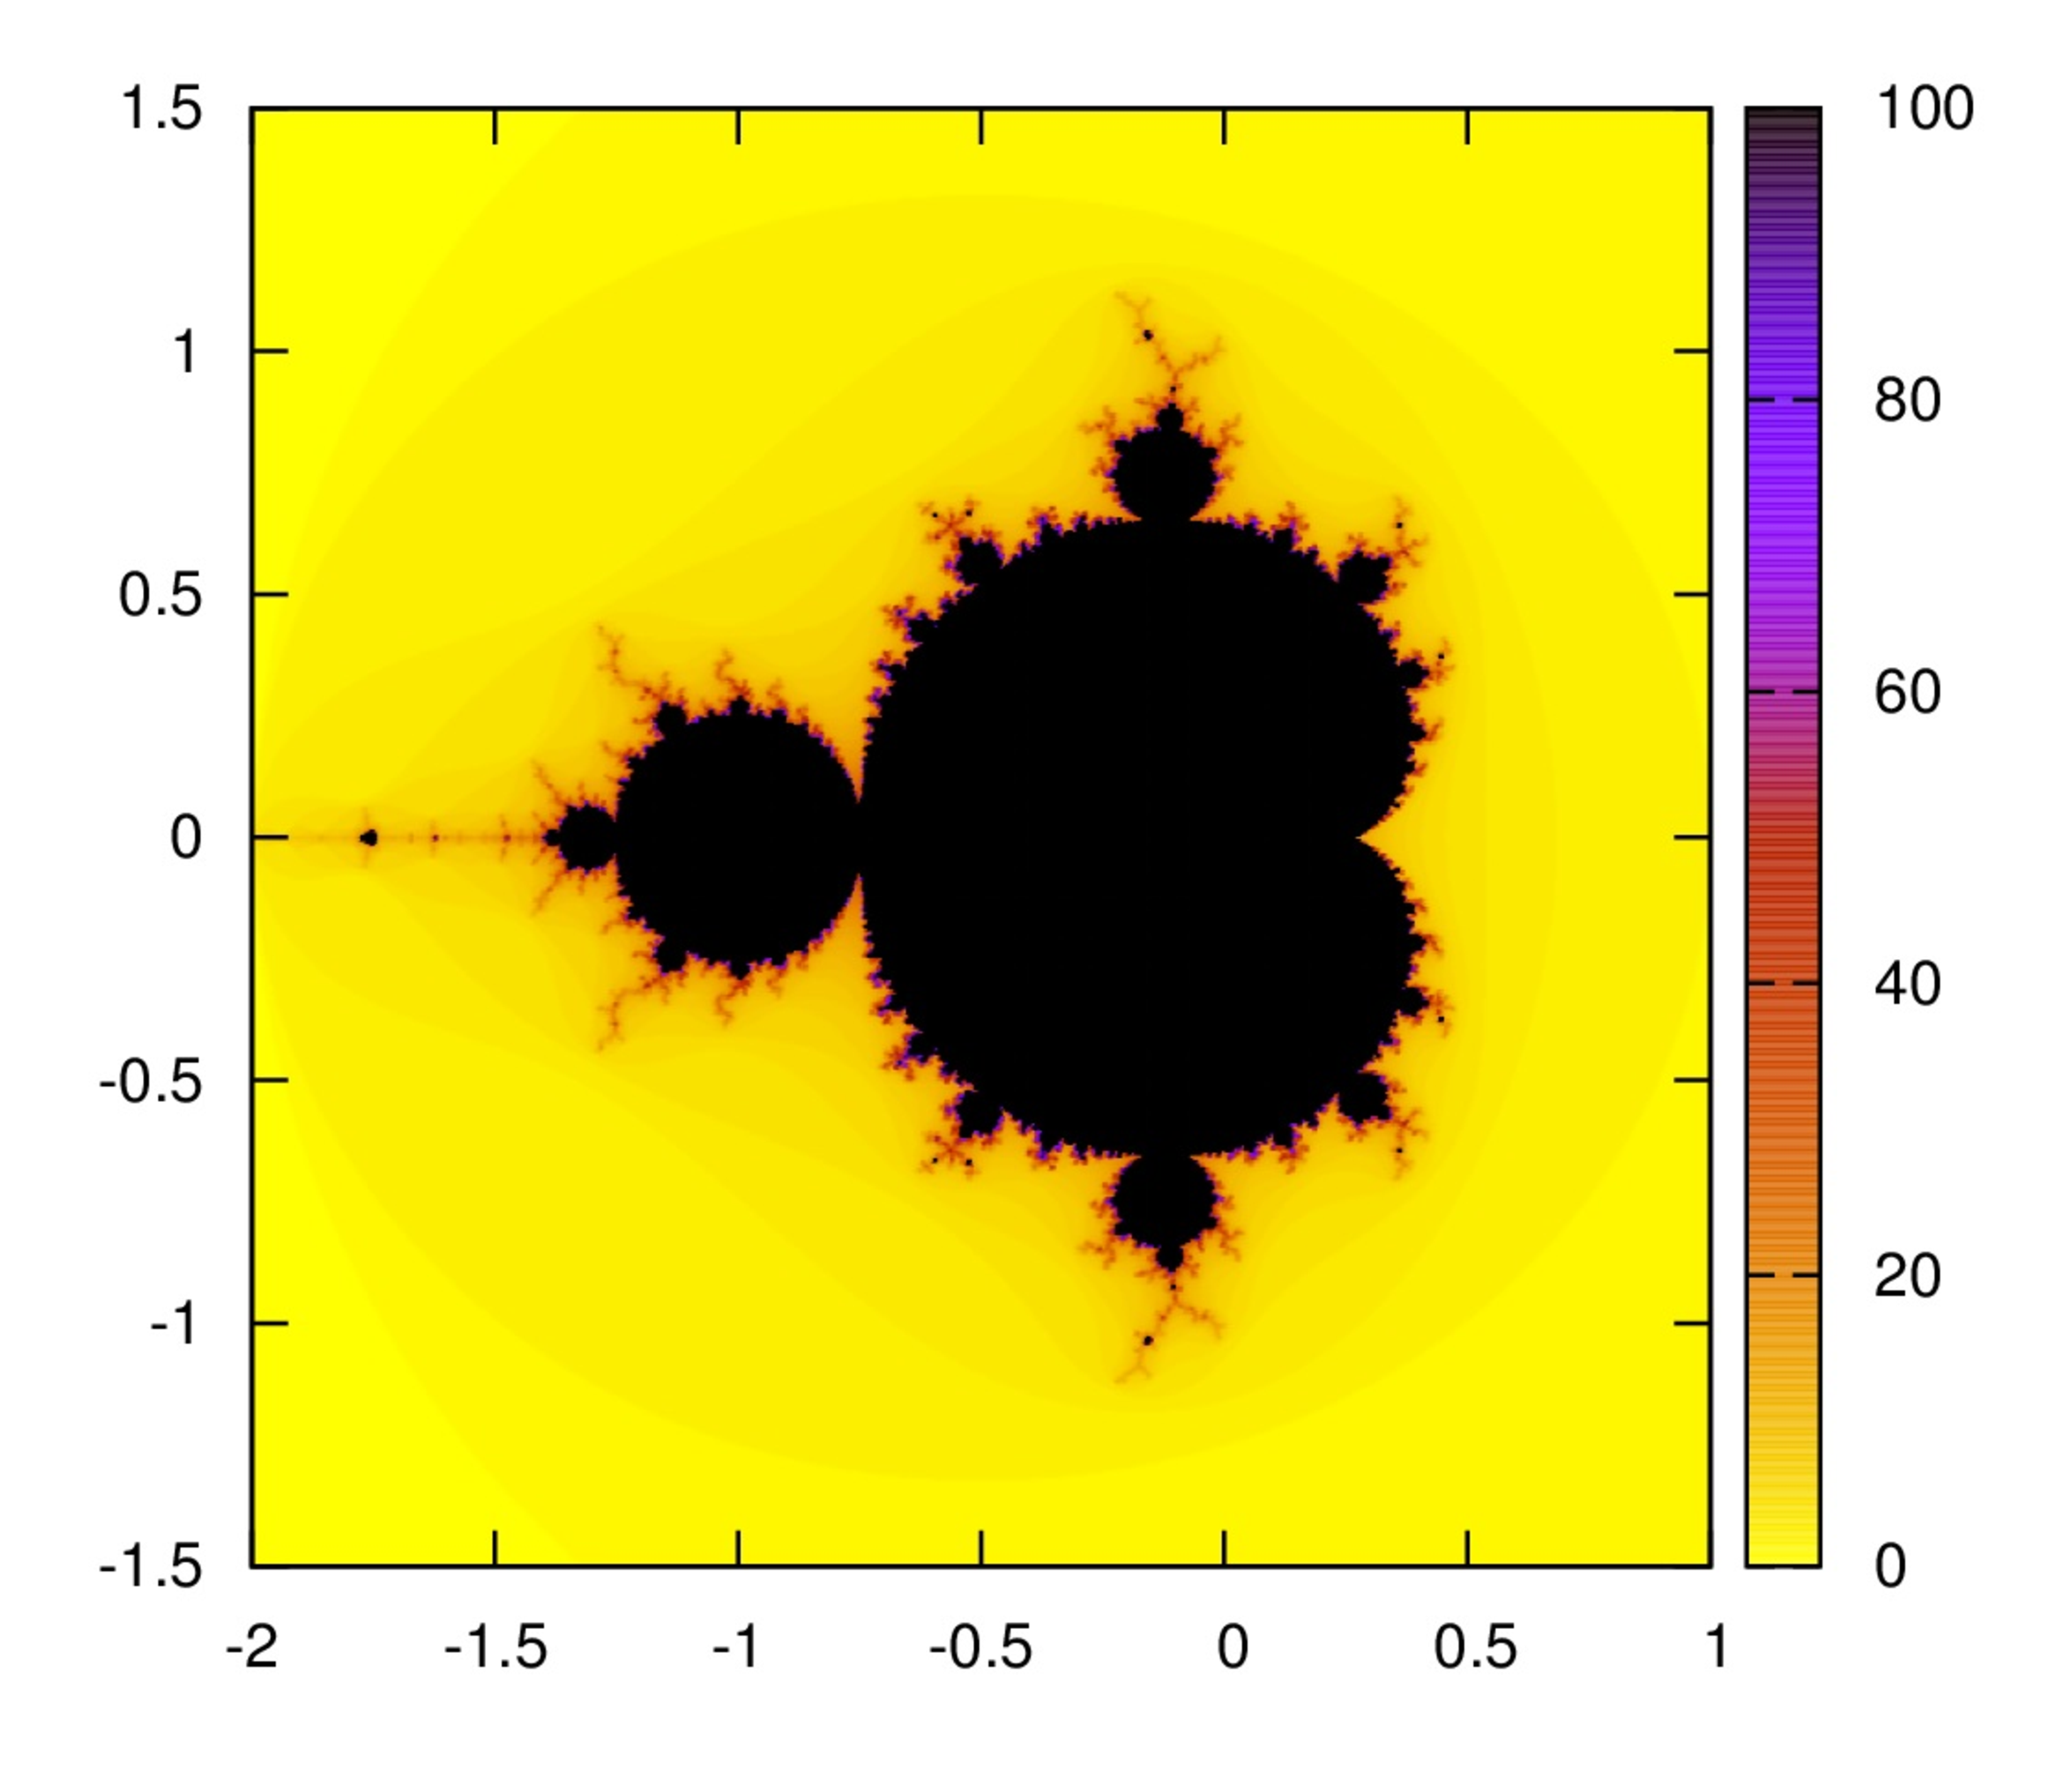
\includegraphics[width=0.75\linewidth]{9_fortran6/figs/mandel}
  \caption{Mandelbrot集合. }
  \end{figure}

  \subsection*{$<$演習課題$>$}
  \begin{enumerate}
  \item 複素数$c$を与え, $|z_N|>2$を満たす最初の$N$を出力するプログラムを作成せよ.
  \item 上のプログラムを改造して, $-2 \le \Re[c] \le 1, -1.5 \le \Im[c] \le 1.5$の範囲における$N$をファイルに出力せよ.
  また, 出力ファイルをカラーマップで描画せよ.
  \item 図形の一部を解像度を上げて再計算し, Mandelbrot集合がフラクタルであることを確かめよ.
  \end{enumerate}


\end{comment}

\chapter{Fortran90の応用2〜数値シミュレーション入門〜}

この章では, これまで学習した知識を用いて初歩的な数値シミュレーションを行う. 
本章と次章を学習することによって, 最終的には, 運動方程式を近似的に解き, 
野球ボールの軌道を計算できるようになることを目標とする. 

多くの数値シミュレーションは, 
解析的に解くことのできない微分方程式を数値的に解く問題に帰着する. 
まずは微分方程式を数値的に解く最も簡単なオイラー法について少し学習し, 
その後, 実際の問題に適用する. 


\section{常微分方程式とオイラー近似}
一階の微分方程式
\begin{equation}
\frac{dx}{dt}=f(x,t)
\end{equation}
を数値的に解くことを考える.
計算機は離散的な値しか扱うことができないので, 微分方程式を差分方程式に近似する.
その最も単純な近似が次のオイラー法である.
\begin{equation}
\frac{x_{n+1}-x_{n}}{\Delta t}=f(x_n,t_n).
\end{equation}
ここで, $\Delta t$を十分に小さい時間刻み幅として,
第$n$ステップにおける$t, x$をそれぞれ$t_n(=n \Delta t), x_n$としている.
初期条件$x(0)=x_0$を与えた上で, $n=0, 1, 2, \cdots$に対して
\begin{equation}
x_{n+1}=x_{n}+f(x_n,t_n)\Delta t
\end{equation}
として逐次$x_n$を求めていく
\footnote
{なお, Taylor展開により,
\begin{equation}
\begin{split}
x(t+\Delta t)&=x(t)+\frac{dx}{dt}(t)\Delta t+O(\Delta t^2)\\
&=x(t)+f(x,t)\Delta t+O(\Delta t^2)
\end{split}
\end{equation}
であるから, Euler法では1ステップあたり$\Delta t^2$程度の誤差が生じることになる. 
このような計算スキームは一次精度と呼ばれる. }. \\

以下の例では, 常微分方程式
\begin{equation}
\frac{dx}{dt}=ax, \ \ \ x(0)=1
\end{equation}
を数値的に解いている.
なお, この方程式の解は
\begin{equation}
x(t)=\exp(at)
\end{equation}
で与えられる.

%TODO サブルーチンを用いる例に変更する. 
\lstinputlisting[caption={Euler法. }, label=eulermethod]{9_fortran6/codes/EulerMethod.f90}

\subsection*{$<$演習課題5.1$>$}
上記の例について, $\Delta t=0.01, 0.1$ および $\Delta t=1.0$ についてそれぞれ計算し, 
その結果を描画することで$\Delta t$の大きさが微分方程式の数値解にどのような影響を及ぼすか考察せよ. 

\section{Lorenz方程式}
気象学者のLorenzは1963年に熱対流の近似モデルとして
以下の方程式を提案した(Lorenz方程式)\footnote{
Lorenz, E. N., ``Deterministic nonperiodic flow", \textit{J. Atms. Sci.} \textbf{20}, pp.130-141, (1963). 
}.
\begin{equation}
\dfrac{dx}{dt}=-ax+ay,
\end{equation}
\begin{equation}
\dfrac{dy}{dt}=\mu x-y-xz,
\end{equation}
\begin{equation}
\dfrac{dz}{dt}=-bz+xy.
\end{equation}
Lorenzは数値計算により, この方程式の解が
不規則で周期性をもたない振動をすることを発見した.
決定論的な微分方程式の解がこのような予測不可能は振舞いを示すことは驚きをもって受け止められ, 
現在ではこのような非周期運動はカオスと呼ばれている.

なお, Lorenz方程式は自明解$x=y=z=0$の他に,
$\mu >1$のとき, 定常解$x=y=\pm \sqrt{b(\mu-1)}, z=\mu-1$をもつ.

\begin{figure}[ht]
\centering
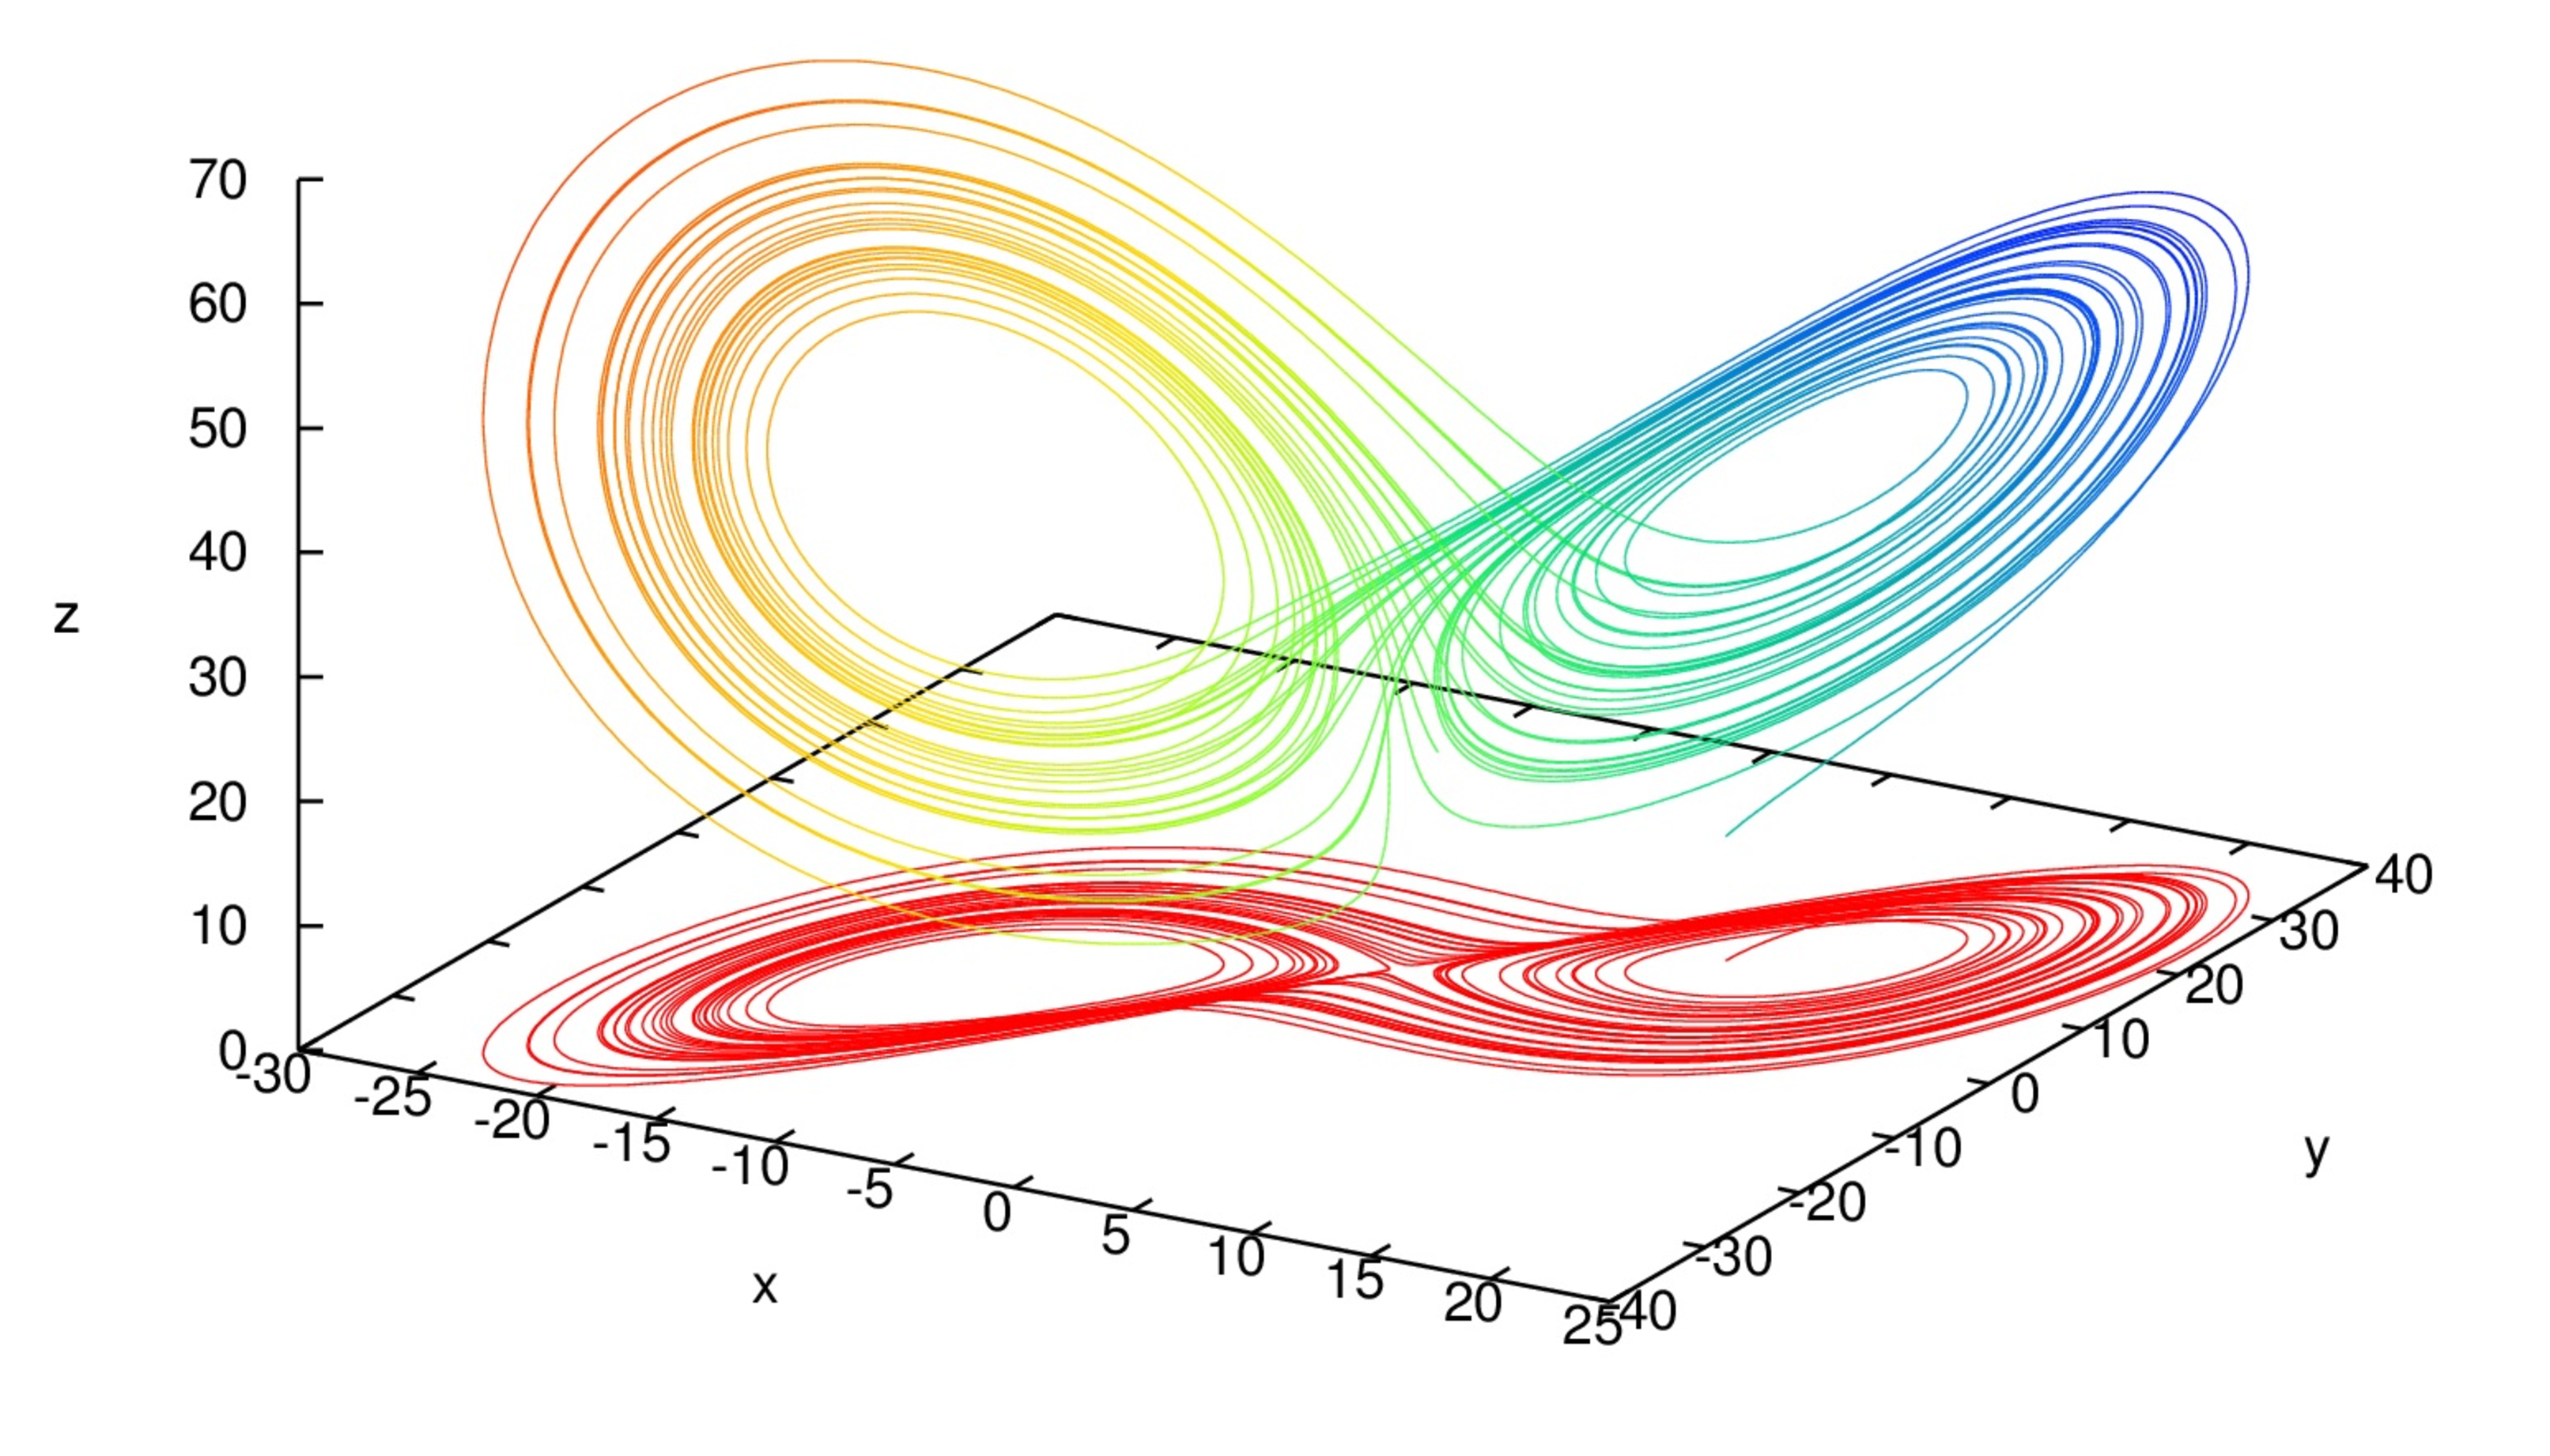
\includegraphics[width=0.9\linewidth]{9_fortran6/figs/lorenz.eps}
\caption{Lorenzアトラクター. }
\end{figure}

\subsection*{$<$演習課題5.2$>$}
\begin{enumerate}
\item $a=10, b=8/3$と固定した上で, Lorenz方程式のシミュレーションを実施せよ.
$\mu$を徐々に増加させ, どのような解が現れるか調べ, 厳密解と比較せよ. 
\item 初期値がわずかに(例えば1\%程度)異なる2ケースのシミュレーション結果を比較せよ.
\end{enumerate}



\chapter{Fortran90の応用3〜運動方程式の解法〜}

前回の演習では一階の連立微分方程式の数値シミュレーションを取り扱った.  
今回はこれを応用して, 二階の微分方程式である運動方程式の解法を学び, 
スポーツの一場面を力学的に解析してみよう. 

\section{物体の自由落下のシミュレーション}
ここでは, 以下のような質点の自由落下をシミュレートする. 
\begin{figure}[ht]
\centering
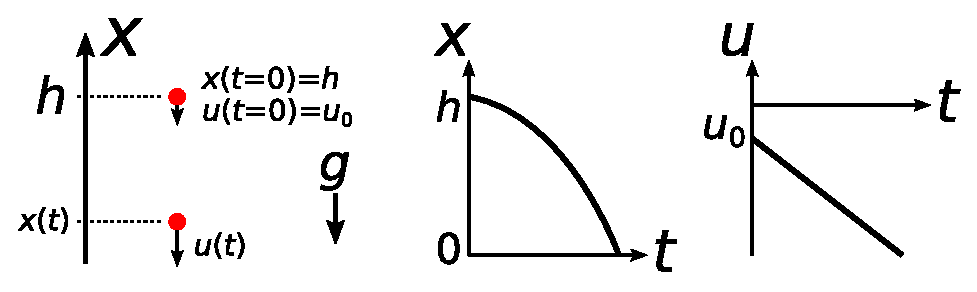
\includegraphics[width=0.8\linewidth]{9_fortran6/figs/freefall.eps}
\caption{自由落下運動の模式図. 時刻$t = 0$ に $x(0)=h$ で鉛直方向に速度$u_0$で
運動している物体(図の赤丸)の軌道をシミュレートする. 
位置$x$および速度$u$の模式図は中・右図のようになる. }
\end{figure}

質点の質量を$m$, 重力加速度を$g$, 初期位置を$h$, 初速を$u_0$とする.
鉛直座標として$x$をとると, 運動方程式は
\begin{equation}
m\frac{d^2x}{dt^2}=-mg, \ \ \ x(0)=h, \ \ \ \frac{dx}{dt}(0)=u_0
\label{eq_freefall}
\end{equation}
で与えられる. 
その解は
\begin{equation}
x(t)=h+u_0t-\frac{1}{2}gt^2.
\end{equation}
であるが, これをコンピュータを用いて近似的に求めてみよう. 

式(\ref{eq_freefall})を以下のように変形することで一階の連立微分方程式が得られる.
\begin{equation}
\frac{dx}{dt}=u, \ \ \ x(0)=h,
\end{equation}
\begin{equation}
\frac{du}{dt}=-g, \ \ \ u(0)=u_0.
\end{equation}
これを前回学習したEuler法を用いて数値的に解けばよい.
プログラムの例を以下に示す.
計算した$x, u$の時間変化をグラフにし, 厳密解と比較してみよ. 

\newpage
\lstinputlisting[caption={質点の自由落下シミュレーション. }, label=freefall]{9_fortran6/codes/FreeFall.f90}

%------------- 空気抵抗下での鉛直落下 ----------------------
\section{空気抵抗下での自由落下のシミュレーション}
上の例では空気抵抗の影響を無視したが, 実際の系では多少なりとも空気抵抗が影響を及ぼす. 
一般に, 空気抵抗は, 物体の速度の大きさの二乗に比例し, その向きと逆方向の力を及ぼす. 
具体的には, 空気抵抗力の大きさ$D$は物体が球形の場合, 
\begin{equation}
D=\frac{1}{2}\rho |\mathbf{u}|^2 \pi a^2 C_D,
\end{equation}
と表せる. 
なお, $|\mathbf{u}|$は速度ベクトル$\mathbf{u}$の絶対値を表す. 
ここで, $\rho$は空気の密度, $a$は球の半径である.
また, 抗力係数$C_D$はある条件\footnote{
Reynolds数$Re=2aU/\nu$ ($\nu$は空気の動粘性係数, $U$は系の代表速度)と呼ばれる無次元数が
$5 \times 10^2 < Re < 1 \times 10^5$のときにこの近似が有効である. 
}
のもとでは約0.44で一定であることが知られている

空気抵抗を考慮した場合, 解くべき微分方程式は, 
\begin{equation}
\frac{dx}{dt}=u, \ \ \ x(0)=h,
\end{equation}
\begin{equation}
\frac{du}{dt}=-g-\frac{D}{m}\frac{u}{|u|}, \ \ \ u(0)=u_0.
\end{equation}
となる. 

空気抵抗の影響を含めた落下運動のシミュレーションを行うソースコードは以下のように書ける. 
計算結果を, 空気抵抗のない場合と比較してみよ. 
\lstinputlisting[caption={空気抵抗下での質点の落下シミュレーション. }, label=freefall]{9_fortran6/codes/FreeFall_friction.f90}

\subsection*{$<$演習課題6.1$>$}
\begin{enumerate}
\item 大きいリンゴと小さいリンゴはどちらが早く落ちるか? リンゴの密度は等しいものとする. 
\item 同じ大きさのリンゴと鉄球はどちらが早く落ちるか?
\item 同じ重さのリンゴと鉄球はどちらが早く落ちるか?
\end{enumerate}

\section{空気抵抗下での野球ボール軌道のシミュレーション}
ここでは, 以下の図に示すような野球ボールの軌道をシミュレートする. 
ここで野球ボールは, 以下のように時刻$t=0$で%原点($x=0, z=0$)から, 
斜め方向に$x, z$方向の速度成分$u_x, u_z$で打ち出される. 

\begin{figure}[ht]
\centering
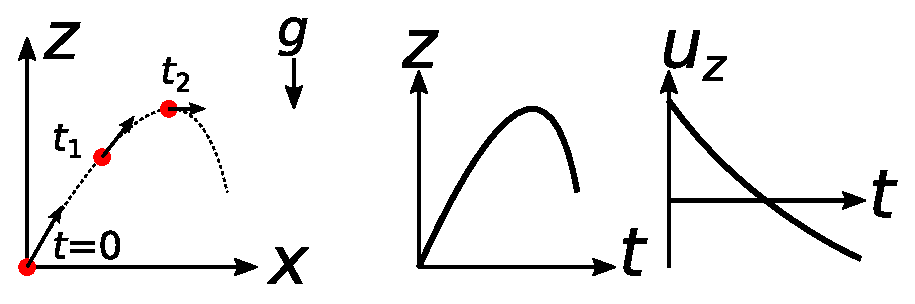
\includegraphics[width=0.8\linewidth]{9_fortran6/figs/shahou.eps}
\caption{野球ボール軌道の模式図. 時刻$t = 0$ に $x(0)=0, z(0)=0$ で
斜め方向に速度$u_x(0), u_z(0)$で打ち出された球状の物体(図の赤丸)が, 
重力および空気抵抗の影響を受けて運動する様子をシミュレートする. 
位置$z$および$z$方向速度$u_z$の模式図は中・右図のようになる. }
\end{figure}

この場合, 空気抵抗の$x, z$方向の成分はそれぞれ
\begin{equation}
  \begin{aligned}
    D_x &= -D u_x / |\mathbf{u}| \\
    D_z &= -D u_z / |\mathbf{u}| \\
  \end{aligned}
\end{equation}
と表される. 

運動方程式は, 速度に関する微分方程式
\begin{equation}
  \begin{aligned}
    \frac{\mathrm{d}u_x}{\mathrm{d}t} &= \frac{D_x}{m},\\
    \frac{\mathrm{d}u_z}{\mathrm{d}t} &= \frac{D_z}{m} - g,\\
  \end{aligned}
\end{equation}
と, 位置に関する微分方程式
\begin{equation}
  \begin{aligned}
    \frac{\mathrm{d}x}{\mathrm{d}t} &= u_x,\\
    \frac{\mathrm{d}z}{\mathrm{d}t} &= u_z,\\
  \end{aligned}
\end{equation}
と表される. 


\if0 %%%%%%%%%%%%%%%%%%%%%%%%%%%%%%%%%%%%%%%%%%%%%%%%%%%%%%%%%%%%%%%
\subsection{Reynolds数が小さい場合}
$Re<0.1$のとき, 抗力係数は理論的に
\begin{equation}
C_D=\frac{24}{Re}
\end{equation}
となることが知られている.

このとき, 運動方程式は
\begin{equation}
m\frac{d^2 x}{dt^2}=-6\pi \rho \nu a \frac{dx}{dt},
\end{equation}
\begin{equation}
m\frac{d^2 y}{dt^2}=-mg-6\pi \rho \nu a \frac{dy}{dt},
\end{equation}
となり, 抵抗は速さの一乗に比例する.
比例係数$6\pi \rho \nu a$は物性値と球の大きさによって決まる.

\begin{table}[h]
\centering
\begin{tabular}{ccc}
\hline
パラメータ & 値 & 備考 \\
\hline
質量$m$ [kg] & - & 適当に与える \\ \hline
半径$a$ [m] & - & 適当に与える \\ \hline
重力加速度$g$ [m/s$^2$] & 9.80665 & - \\ \hline
空気の密度$\rho$[kg/m$^3$] & 1.261 & 280Kの場合 \\
 & 1.176 & 300Kの場合 \\ \hline
空気の動粘性係数$\nu$[m$^2$/s] & 1.395 $\times 10^{-5}$ & 280Kの場合 \\
 & 1.579 $\times 10^{-5}$ & 300Kの場合 \\ \hline
水の密度$\rho$[kg/m$^3$] & 9.999 $\times 10^2$ & 280Kの場合 \\
 & 9.966 $\times 10^2$ & 300Kの場合 \\ \hline
水の動粘性係数$\nu$[m$^2$/s] & 1.436 $\times 10^{-6}$ & 280Kの場合 \\
 & 8.574 $\times 10^{-7}$ & 300Kの場合 \\ \hline
Reynolds数$Re$[-] & $\frac{2aU}{\nu}$ & 計算する \\ \hline
抗力係数$C_D$[-] & $\frac{24}{Re}$ & $Re<0.1$における理論式 \\
& $(\sqrt{\frac{24}{Re}}+0.5407)^2$ & $Re< 6000$における経験式 \\
& $0.44$ & $5 \times 10^2 < Re < 1 \times 10^5$における近似値 \\
& & (この範囲で抵抗は速度の二乗に比例) \\ \hline
スケールハイト$H_\rho$[m] & 8 $\times 10^3$ & 実際は温度によって変化する \\ \hline
\end{tabular}
\end{table}
\fi %%%%%%%%%%%%%%%%%%%%%%%%%%%%%%%%%%%%%%%%%%%%%%%%%%%%%%%%%%%%%%%%

\subsection*{$<$演習課題6.2$>$}
大谷翔平は野球ボールを最大球速 165km/h で投げることができる. 
彼は地面に対しどの方向(角度$\theta$)に対してもこの初速で野球ボールを投げ出すことができ, 
彼の身長は193cmで腕の長さは85cmとする. 
また, ボールの回転は考慮しないものとする. 

これら仮定のもとで, 以下の状況をシミュレート	せよ. 
\begin{enumerate}
% TODO 問題が難しすぎる気がする. 
\item 空気抵抗がない場合($C_D=0$), 適当な角度$\theta$に対するシミュレーションをおこない, 解析解と比較せよ. 
ボールのリリース点の高さは適当に設定すること. 
\item 空気抵抗がある場合のシミュレーションをおこない, 空気抵抗がない場合と比較せよ.
\end{enumerate}


各物理量の具体的な値については, 以下の表を参考にするとよい.
%その他, 必要なパラメータがあれば各自調べること. 
\begin{table}[H]
\centering
\begin{tabular}{ccc}
\hline
パラメータ & 値 & 備考 \\
\hline
質量$m$ [kg] & 0.145 & 野球ボール \\ \hline
半径$a$ [m] & 0.036 &  野球ボール \\ \hline
重力加速度$g$ [m/s$^2$] & 9.80665 & - \\ \hline
空気の密度$\rho$[kg/m$^3$] & 1.261 & 280Kの場合 \\
 & 1.176 & 300Kの場合 \\ \hline
空気の動粘性係数$\nu$[m$^2$/s] & 1.395 $\times 10^{-5}$ & 280Kの場合 \\
 & 1.579 $\times 10^{-5}$ & 300Kの場合 \\ \hline
抗力係数$C_D$[-] & $0.44$ & $5 \times 10^2 < Re < 1 \times 10^5$のとき \\ \hline
Reynolds数$Re$[-] & - & $2aU/\nu$ \\ \hline
\end{tabular}
\end{table}



\subsection*{$<$演習課題6.3$>$}
空気抵抗のもとでの放物運動が関係するスポーツシーンを何でもよいので一つ取り上げ, 適当な問題設定に対するシミュレーションを実施せよ. 
この問題は本質的には二次元問題であるが, 三次元の運動方程式を書き下しておくと, 

\begin{equation}
  \begin{aligned}
    \frac{\mathrm{d}x}{\mathrm{d}t} &= u_x,\\
    \frac{\mathrm{d}y}{\mathrm{d}t} &= u_y,\\
    \frac{\mathrm{d}z}{\mathrm{d}t} &= u_z,\\
    \frac{\mathrm{d}u_x}{\mathrm{d}t} &= \frac{D_x}{m},\\
    \frac{\mathrm{d}u_y}{\mathrm{d}t} &= \frac{D_y}{m},\\
    \frac{\mathrm{d}u_z}{\mathrm{d}t} &= \frac{D_z}{m} - g\\
  \end{aligned}
\end{equation}
となる. ここで, 空気抵抗の$x, y, z$方向の成分はそれぞれ
\begin{equation}
  \begin{aligned}
    D_x &= -D u_x / |\mathbf{u}| \\
    D_y &= -D u_y / |\mathbf{u}| \\
    D_z &= -D u_z / |\mathbf{u}| \\
  \end{aligned}
\end{equation}
である. 

\begin{itemize}
\item[例1. ]野球ボールを最も遠くまで飛ばすためには, 
大谷翔平は地面に対しどの角度で野球ボールを投げる必要があるか. 
\item[例2. ]大谷翔平が投げたボールがストライクになるためには, どのような角度で投げればよいか. 
初速, ピッチャーとキャッチャーの距離やストライクゾーンの広さは適当に設定せよ. 
\item[例3. ]サッカーのフリーキックで壁を越えてゴールに入れるにはどのような初速, 角度で蹴ればよいか. 
ゴールまでの距離や壁の高さは自由に設定せよ. 
\item[例4. ]バスケットボールのフリースローを成功させるにはどのような初速, 角度で投げればよいか. 
リリース点の高さやゴールの高さ・リングの直径などは自由に設定せよ. 
\end{itemize}



\chapter{演習課題}
これまで数週にわたってFortranプログラミングを学習してきたが, 
単にプログラムを書いて, 出力された結果をもとに図を描いただけでは社会に対するアウトプットとならない. 
解くべき問題の背景, 問題へのアプローチの仕方, 得られた結果とそれがもつ意味, さらなる問題提起, について
日本語(あるいは英語)でまとめる技術は卒業までに身につけなければならないスキルである. 

\section{科学技術レポート}
これまでのプログラミング課題の中から好きなものを一つ取り上げ, Wordを用いてレポートとしてまとめよ. 
レポートには次の内容を含めること. (各章の題目は以下のものに限定しないが, 参考までに列挙している)

\begin{enumerate}
\item 序論, 緒言, イントロダクション, はじめに, 背景

選んだ問題の背景について述べ, 本レポートにて解くべき問題と目的について述べる. 

\item 数値計算法, 数値解析手法, 数値シミュレーション, アルゴリズム

設定した問題を解くための手法について述べる. 
基礎方程式やアルゴリズム, 設定したパラメータ等についてまとめる. 
必要に応じて, 問題のポンチ絵やプログラムの流れを示すフローチャートを用いる. 
第三者であってもレポートを読めば, 数値計算結果を再現できるように詳細に記述する. 


\item 結果, 数値計算結果, 結果と考察

得られた結果を図や表を用いて示す. 
単に図表を並べるだけではなく, それぞれの図表が意味するものを言葉を用いて丁寧に記述する. 
また, 図には縦軸横軸のラベル, 凡例, キャプション等を必ずつけること. 
有次元量には必ず単位が必要であることに注意せよ. 

なお, 得られた結果の妥当性についてもここで言及する. 

\item 結論, 結言, まとめ, おわりに

レポートの内容を簡潔にまとめ, さらなる問題提起(現状の解析の問題点など)をおこなう. 

\item 参考文献

参考にした文献がある場合には, 必ず参考文献リストを付ける. 
通常は教科書や論文を列挙するが, 
本レポートに関してはWebページ上の情報であってもよい. 
その場合, URLと最終アクセス日時を記すこと. 

\end{enumerate}

\section{科学技術プレゼンテーション}
Wordでまとめたものと同じテーマについて, PowerPointを用いてまとめよ. 
スライドには少なくとも1ページずつ次の内容を含め, 全部で5-10ページ程度にまとめること. 

\begin{enumerate}
\item 表紙

\item 序論, 緒言, イントロダクション, はじめに, 背景

\item 数値計算法, 数値解析手法, 数値シミュレーション, アルゴリズム

\item 結果, 数値計算結果, 結果と考察

\item 結論, 結言, まとめ, おわりに


\end{enumerate}

%\chapter{Fortran90の応用1〜数値計算の高速化〜}

%以上のように,
コンピュータによる数値計算は, 手計算では解を求めることができないような複雑な問題であっても,
計算誤差の範囲内で近似的に解くことができるため, 現代の科学技術を支える非常に強力な手段である.
しかしながら, 多くの場合, すぐに計算量が膨大になり, 現実的な時間内に計算が終わらなくなってしまう. 
それを克服するためには, アルゴリズムを工夫して意味のない計算を省略するなどして,
計算時間を短くすることが必要である.

この章では``素数の探索''という簡単な例を用いて, 数値計算の高速化を体験する.


\section{素数探索}
素数とは1と自分以外に約数をもたない自然数のことである.
ここでは, 計算機を用いて膨大な数の素数をいかに速く求めるかを目指す.

\subsection*{$<$演習課題4.1$>$}
\begin{enumerate}
\item ある自然数$n$を与え, それを$n-1$までの自然数で割り算することにより,
$n$が素数かどうかを判定するプログラムを作成せよ.
(ヒント: 余りを計算する関数\verb|mod|を利用する)
\item 上記のプログラムをサブルーチン化し, 100,000番目の素数の値を求めるプログラムを作成せよ.
\end{enumerate}

\subsection{実行速度の計測}
次に, 上で作成したプログラムの高速化に取り組む.

プログラムの高速化を行うためには, やみくもに試行錯誤を行なうのではなく,
どの計算に時間がかかっているか(ホットスポットと呼ばれる)を調べ,
多くの計算時間が費やしている部分を重点的に改善することが必要である.

プログラムの実行時間は, \verb|system_clock|関数により得ることができる.
以下に, 計算時間を計測するプログラムの一例を示す.

\lstinputlisting[caption={実行時間の測定. }, label=timing]{8_fortran5/codes/Timing.f90}


\subsection*{$<$演習課題4.2$>$}
\begin{enumerate}
\item 100,000番目の素数の探索にかかった時刻を計測するプログラムを作成せよ.
\item $i$番目の素数の探索にかかった時間$t(i)$をグラフに描画し,
その様子から素数探索にかかる時間の特徴を考察せよ.
\item 上での考察を元にアルゴリズムを工夫して, 100,000番目の素数を探索する高速なプログラムを作成せよ.
\end{enumerate}







\begin{comment}
  \section{素数探索}

  以下にプログラム例を示す.
  %TODO 実行時間を測れる例に変更する.
  %TODO 特にわかりやすい例として, ファイルへの書き込みを毎回行っておく.



  \section{Mandelbrot集合}
  Mandelbrot集合とは,
  \begin{equation}
  z_{n+1}=z_n^2+c, \ \ \ z_0=0
  \end{equation}
  という漸化式で定義される複素数列$z_n$が$n \to \infty$の極限で発散しないという
  条件を満たす複素数$c$の集合である.
  Mandelbrot集合はその一部が全体と相似であり, フラクタルと呼ばれる.

  $|z_n|>2$のとき, $|z_{n+1}/z_n|>1$となることが示されるので(証明略),
  複素数列が発散する条件はある$N$に対して$|z_N|>2$となることである.

  \begin{figure}[ht]
  \centering
  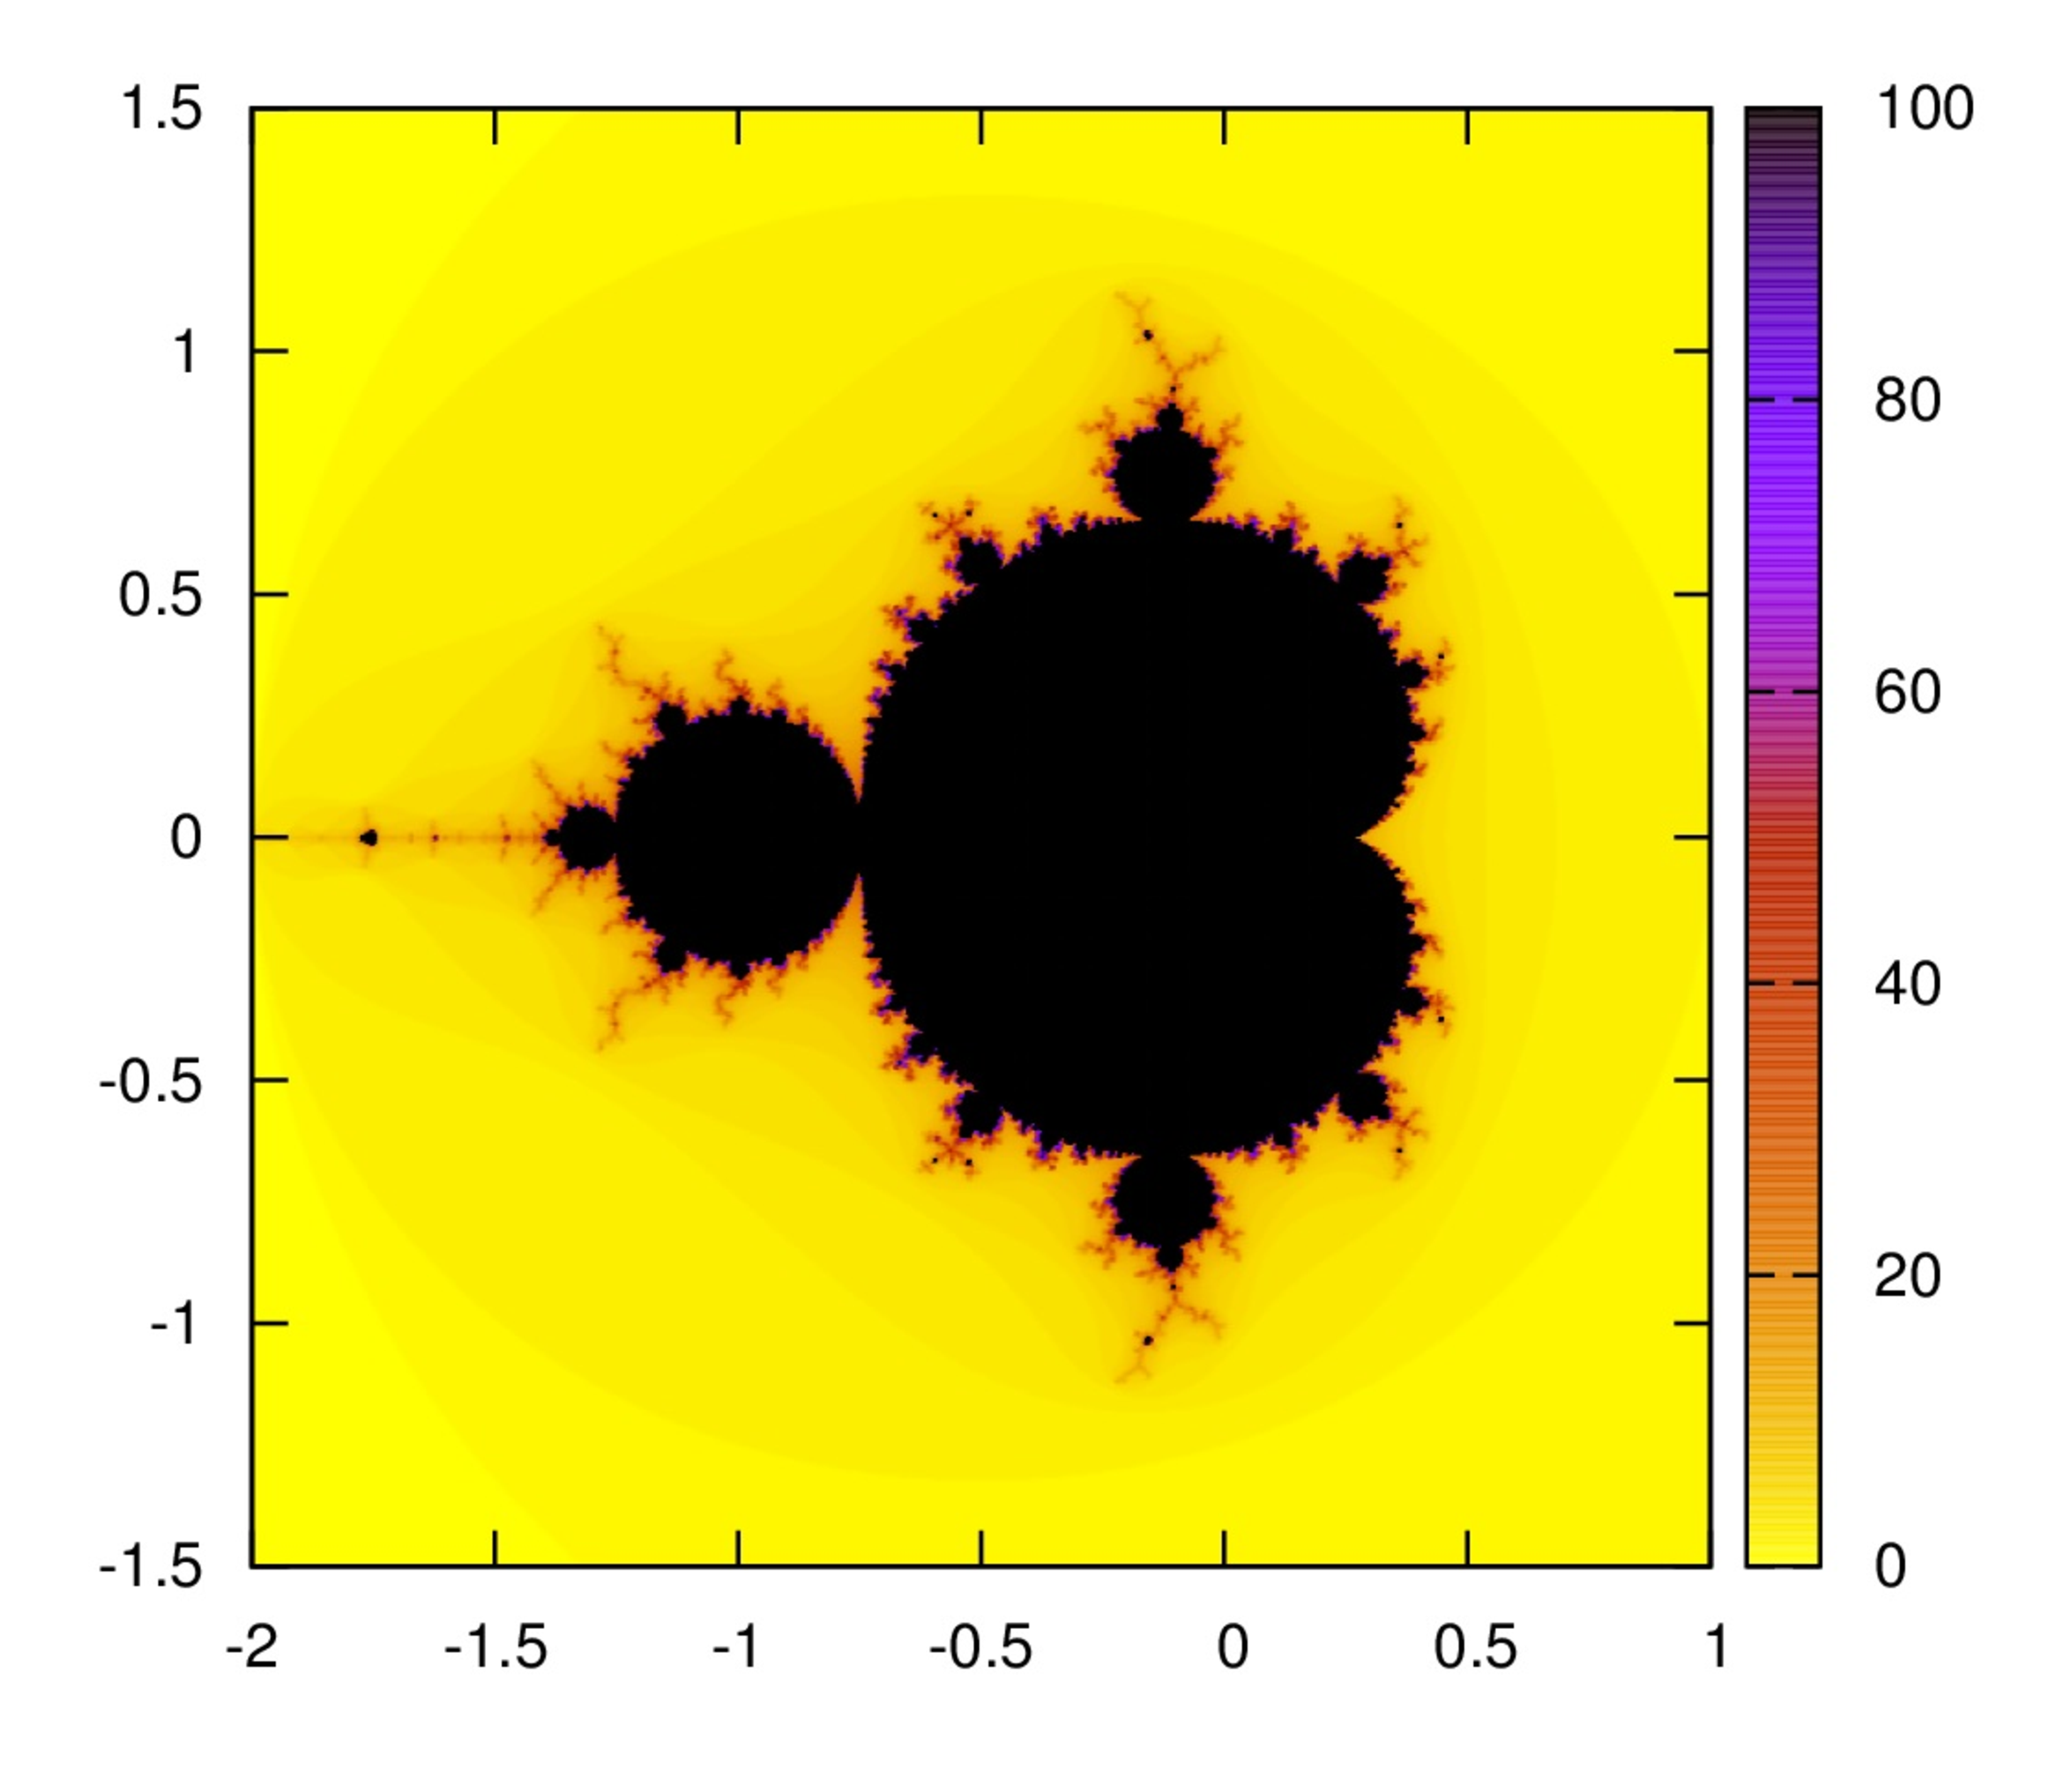
\includegraphics[width=0.75\linewidth]{9_fortran6/figs/mandel}
  \caption{Mandelbrot集合. }
  \end{figure}

  \subsection*{$<$演習課題$>$}
  \begin{enumerate}
  \item 複素数$c$を与え, $|z_N|>2$を満たす最初の$N$を出力するプログラムを作成せよ.
  \item 上のプログラムを改造して, $-2 \le \Re[c] \le 1, -1.5 \le \Im[c] \le 1.5$の範囲における$N$をファイルに出力せよ.
  また, 出力ファイルをカラーマップで描画せよ.
  \item 図形の一部を解像度を上げて再計算し, Mandelbrot集合がフラクタルであることを確かめよ.
  \end{enumerate}


\end{comment}

%\chapter{Fortran90の応用2〜数値シミュレーション入門〜}

この章では, これまで学習した知識を用いて初歩的な数値シミュレーションを行う. 
本章と次章を学習することによって, 最終的には, 運動方程式を近似的に解き, 
野球ボールの軌道を計算できるようになることを目標とする. 

多くの数値シミュレーションは, 
解析的に解くことのできない微分方程式を数値的に解く問題に帰着する. 
まずは微分方程式を数値的に解く最も簡単なオイラー法について少し学習し, 
その後, 実際の問題に適用する. 


\section{常微分方程式とオイラー近似}
一階の微分方程式
\begin{equation}
\frac{dx}{dt}=f(x,t)
\end{equation}
を数値的に解くことを考える.
計算機は離散的な値しか扱うことができないので, 微分方程式を差分方程式に近似する.
その最も単純な近似が次のオイラー法である.
\begin{equation}
\frac{x_{n+1}-x_{n}}{\Delta t}=f(x_n,t_n).
\end{equation}
ここで, $\Delta t$を十分に小さい時間刻み幅として,
第$n$ステップにおける$t, x$をそれぞれ$t_n(=n \Delta t), x_n$としている.
初期条件$x(0)=x_0$を与えた上で, $n=0, 1, 2, \cdots$に対して
\begin{equation}
x_{n+1}=x_{n}+f(x_n,t_n)\Delta t
\end{equation}
として逐次$x_n$を求めていく
\footnote
{なお, Taylor展開により,
\begin{equation}
\begin{split}
x(t+\Delta t)&=x(t)+\frac{dx}{dt}(t)\Delta t+O(\Delta t^2)\\
&=x(t)+f(x,t)\Delta t+O(\Delta t^2)
\end{split}
\end{equation}
であるから, Euler法では1ステップあたり$\Delta t^2$程度の誤差が生じることになる. 
このような計算スキームは一次精度と呼ばれる. }. \\

以下の例では, 常微分方程式
\begin{equation}
\frac{dx}{dt}=ax, \ \ \ x(0)=1
\end{equation}
を数値的に解いている.
なお, この方程式の解は
\begin{equation}
x(t)=\exp(at)
\end{equation}
で与えられる.

%TODO サブルーチンを用いる例に変更する. 
\lstinputlisting[caption={Euler法. }, label=eulermethod]{9_fortran6/codes/EulerMethod.f90}

\subsection*{$<$演習課題5.1$>$}
上記の例について, $\Delta t=0.01, 0.1$ および $\Delta t=1.0$ についてそれぞれ計算し, 
その結果を描画することで$\Delta t$の大きさが微分方程式の数値解にどのような影響を及ぼすか考察せよ. 

\section{Lorenz方程式}
気象学者のLorenzは1963年に熱対流の近似モデルとして
以下の方程式を提案した(Lorenz方程式)\footnote{
Lorenz, E. N., ``Deterministic nonperiodic flow", \textit{J. Atms. Sci.} \textbf{20}, pp.130-141, (1963). 
}.
\begin{equation}
\dfrac{dx}{dt}=-ax+ay,
\end{equation}
\begin{equation}
\dfrac{dy}{dt}=\mu x-y-xz,
\end{equation}
\begin{equation}
\dfrac{dz}{dt}=-bz+xy.
\end{equation}
Lorenzは数値計算により, この方程式の解が
不規則で周期性をもたない振動をすることを発見した.
決定論的な微分方程式の解がこのような予測不可能は振舞いを示すことは驚きをもって受け止められ, 
現在ではこのような非周期運動はカオスと呼ばれている.

なお, Lorenz方程式は自明解$x=y=z=0$の他に,
$\mu >1$のとき, 定常解$x=y=\pm \sqrt{b(\mu-1)}, z=\mu-1$をもつ.

\begin{figure}[ht]
\centering
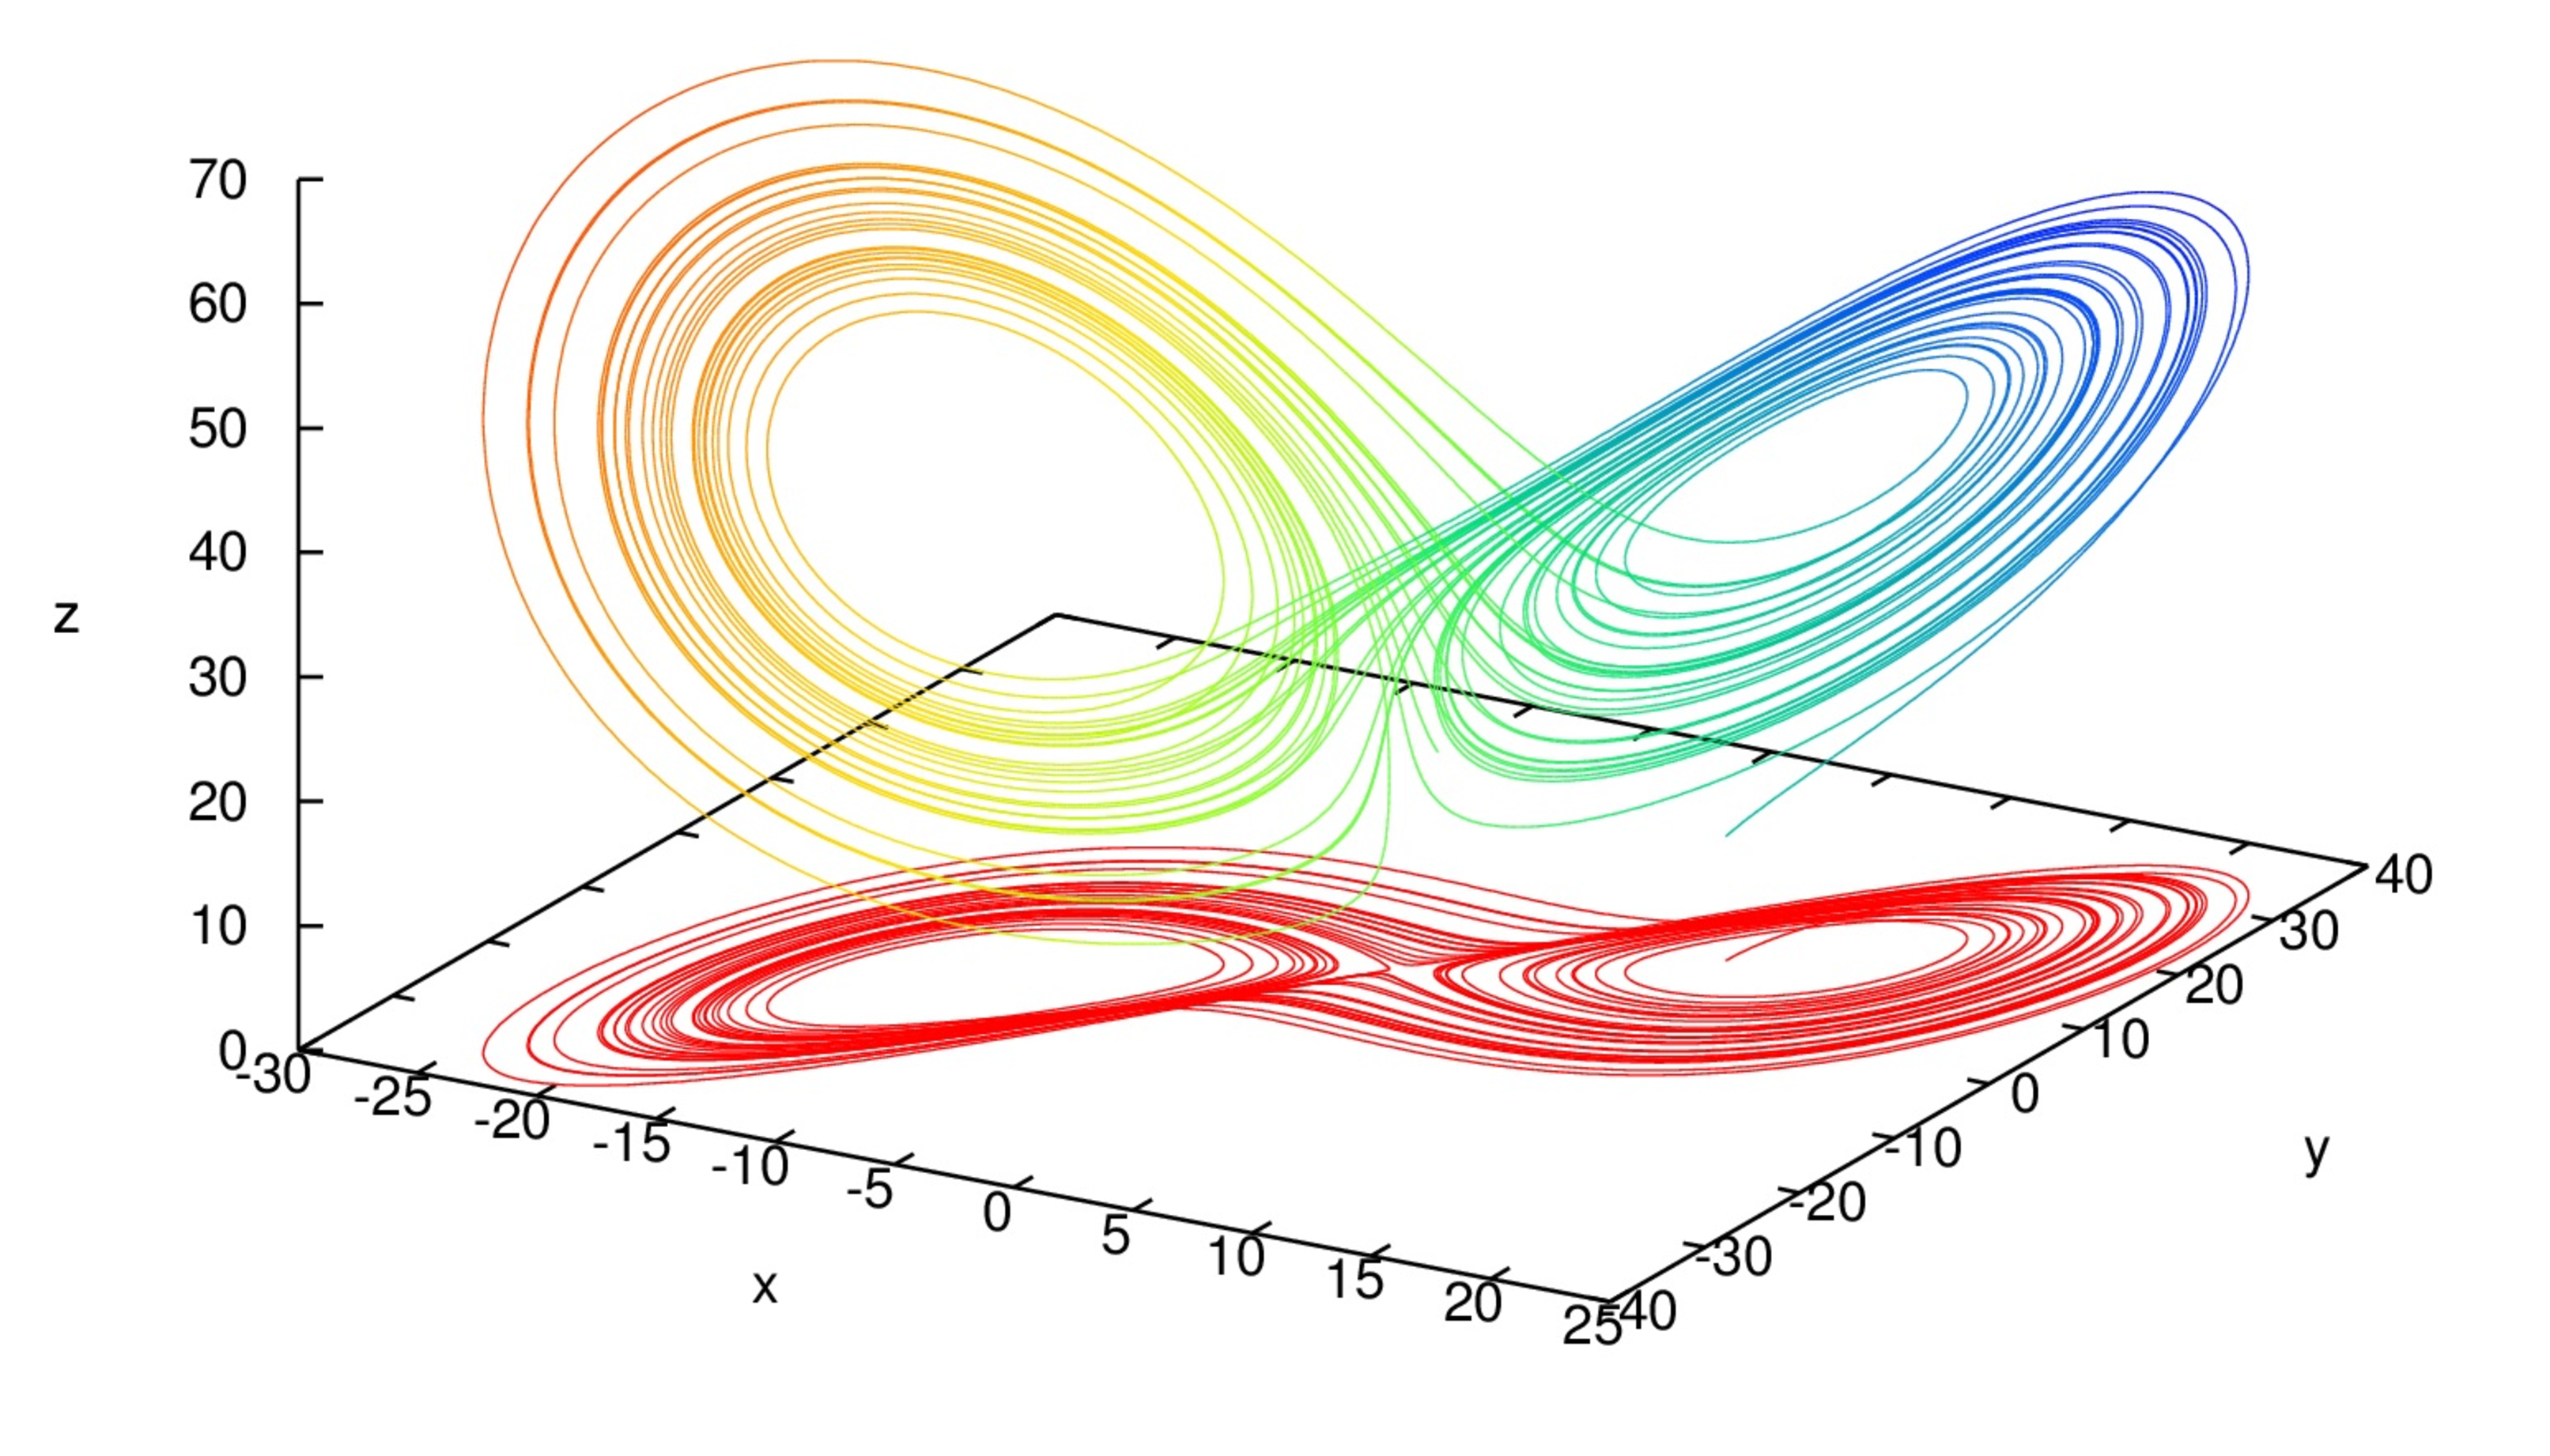
\includegraphics[width=0.9\linewidth]{9_fortran6/figs/lorenz.eps}
\caption{Lorenzアトラクター. }
\end{figure}

\subsection*{$<$演習課題5.2$>$}
\begin{enumerate}
\item $a=10, b=8/3$と固定した上で, Lorenz方程式のシミュレーションを実施せよ.
$\mu$を徐々に増加させ, どのような解が現れるか調べ, 厳密解と比較せよ. 
\item 初期値がわずかに(例えば1\%程度)異なる2ケースのシミュレーション結果を比較せよ.
\end{enumerate}



\backmatter
% bibliography, glossary and index would go here.
\appendix
\section{gfortranのインストール}
gfortranはフリーのコンパイラであるから, 
自分のもっているノートPCや家にあるPCにインストールしておくのがよい. 
その手順を以下に記す. 

\begin{enumerate}
\item https://sourceforge.net/projects/mingw-w64/ にアクセスし, mingw-w64-install.exeをダウンロードする. 
\item ダウンロードしたmingw-w64-install.exeを実行する. 
\item 図\ref{fig_install}(a)で[Next]を押す. 
\item 図\ref{fig_install}(b)でVersionは5.2.0以降, Architectureは64bitマシンの場合はx86\_64を選択する. それ以外の項目はデフォルトでよい. 
\item 図\ref{fig_install}(c)でインストール先を聞かれるが, デフォルトでよい. 
\item 図\ref{fig_install}(d)のようにインストールが始まるのでしばらく待つ.  
\item 図\ref{fig_install}(e)で[Next]を押す. 
\item 図\ref{fig_install}(f)の画面が出たらインストールは終了である. 
\item インストールしたgfortranをコマンドプロンプトから実行するにはgfortranをインストールしたディレクトリにパスを通しておく必要がある.
\textcolor{red}{環境変数の設定を失敗するとシステムが正常に動作しなくなる可能性がある. 自己責任で慎重におこなうこと. }

[コントロールパネル]$\to$[システム]$\to$[システムの詳細設定]$\to$[環境変数]を開く. 
\item システム環境変数中のPathを選択し, [編集]を押す. 
\item 変数値の末尾にセミコロン(;)を挿入し, 続けて各自がgfortranをインストールしたディレクトリを追加する. 
アドレスバーをコピーし, そのまま貼り付けるのがよい. 次はその例である. 

C:Y\llap{=}Program FilesY\llap{=}mingw-w64Y\llap{=}x86\_64-6.1.0-posix-seh-rt\_v5-rev0Y\llap{=}mingw64Y\llap{=}bin

\item コマンドプロンプトを立ち上げ, gfortranとタイプする. 画面に no input files と表示されれば, 正しくパスが通っている. 
\end{enumerate}

\begin{figure}[ht]
\centering
\subfloat[]{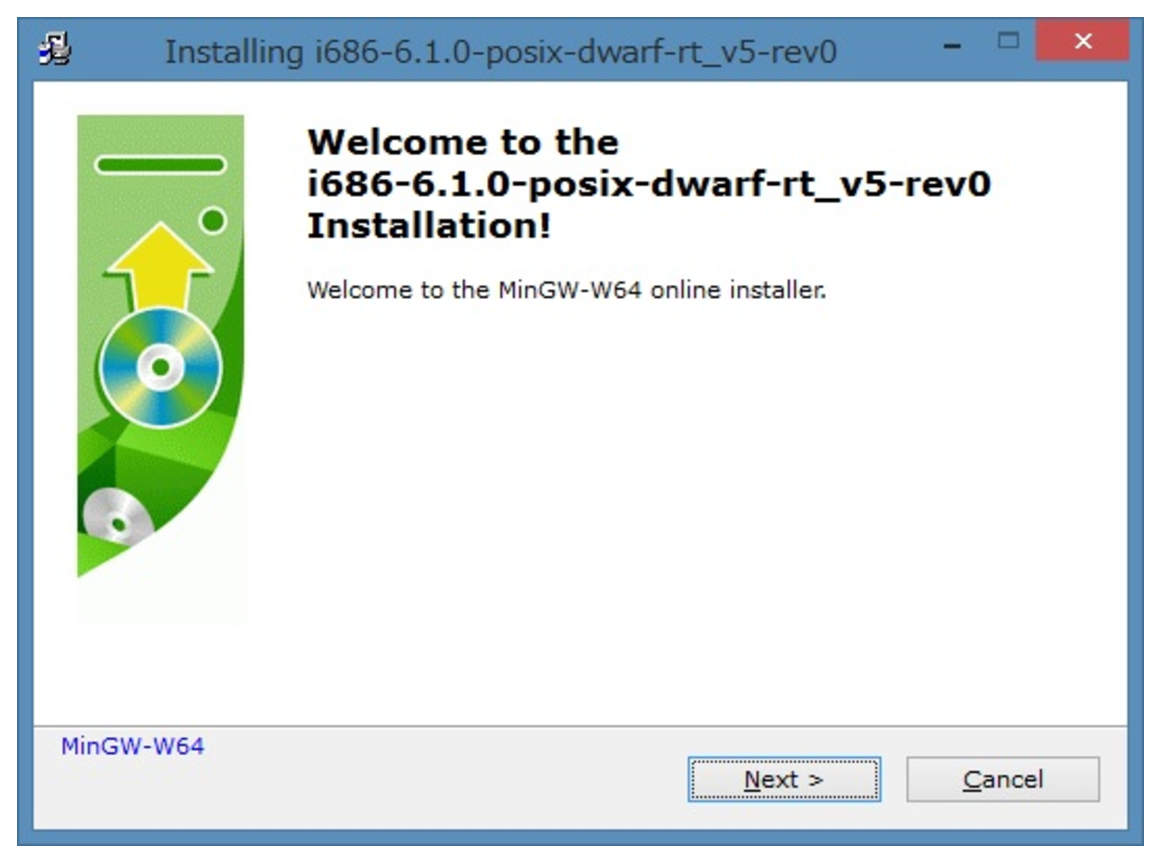
\includegraphics[width=0.45\linewidth]{appendix/install/1/install1.eps}} \hspace{5mm}
\subfloat[]{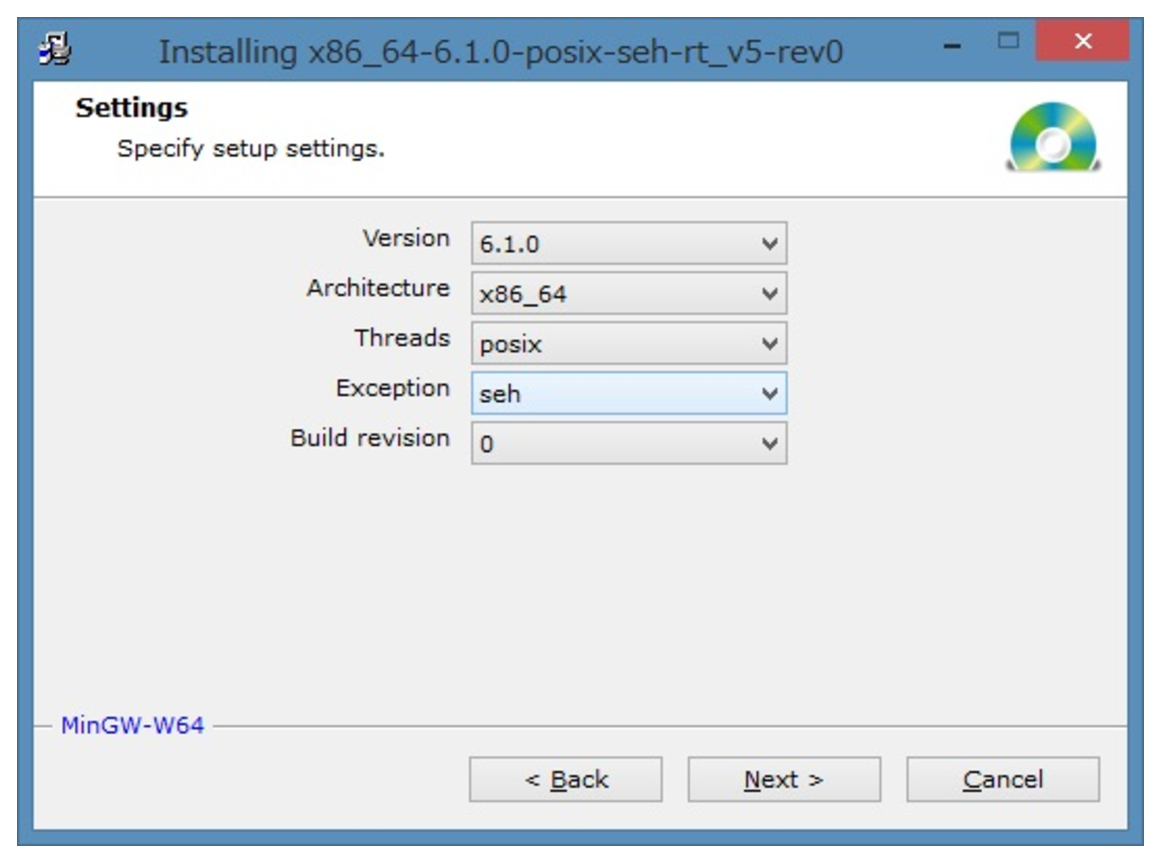
\includegraphics[width=0.45\linewidth]{appendix/install/1/install2.eps}}\\
\subfloat[]{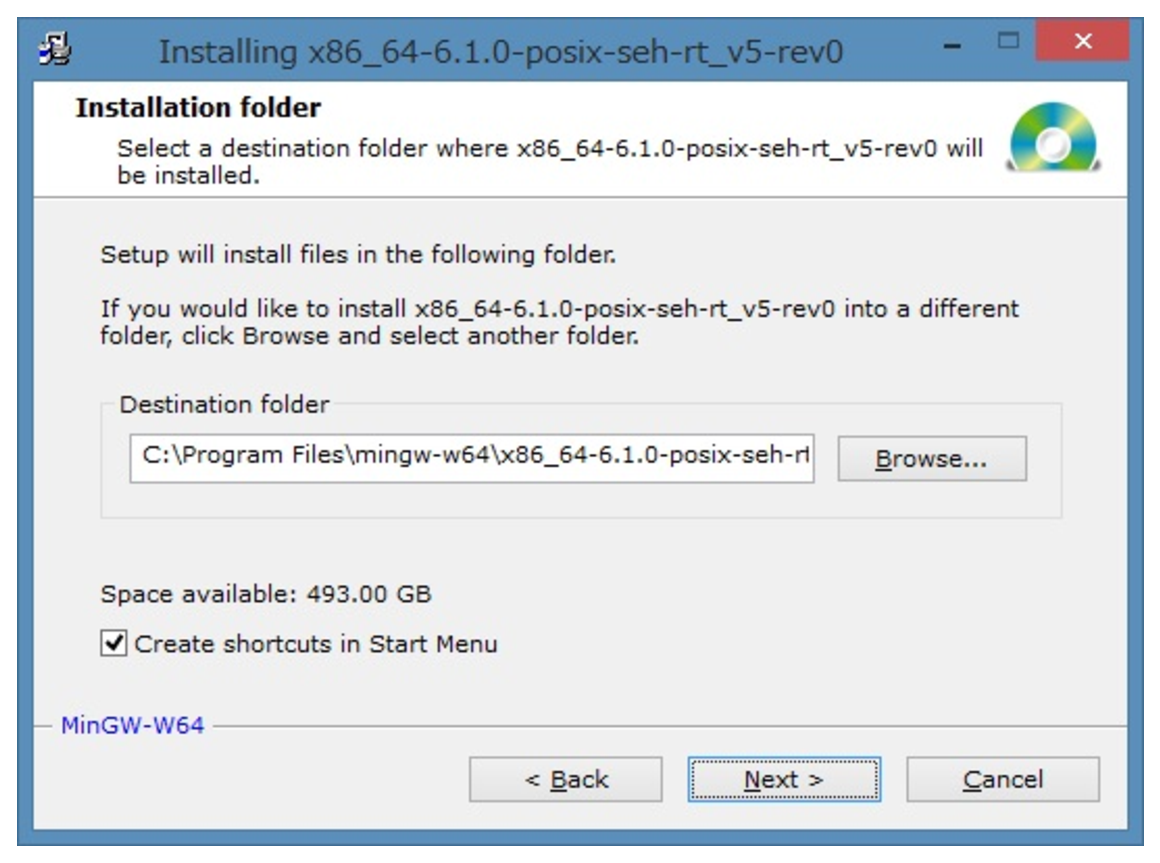
\includegraphics[width=0.45\linewidth]{appendix/install/1/install3.eps}} \hspace{5mm}
\subfloat[]{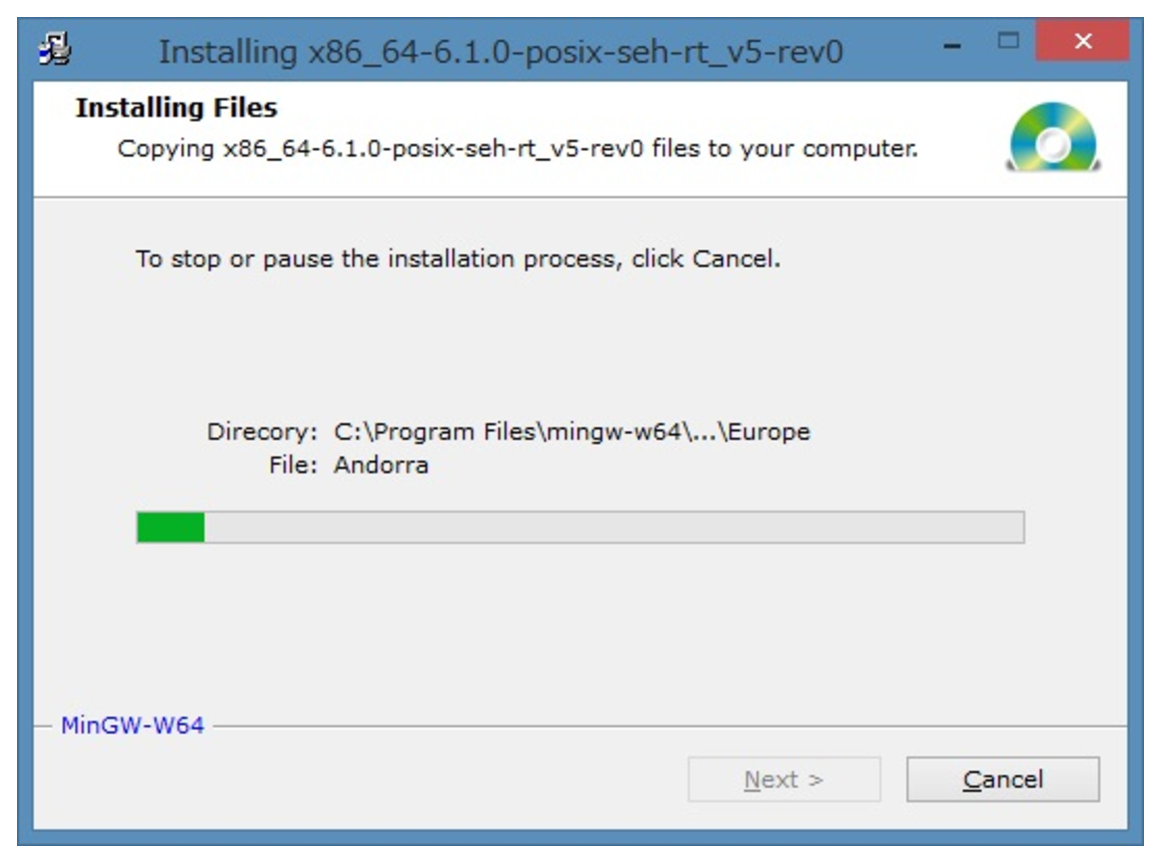
\includegraphics[width=0.45\linewidth]{appendix/install/1/install4.eps}}\\
\subfloat[]{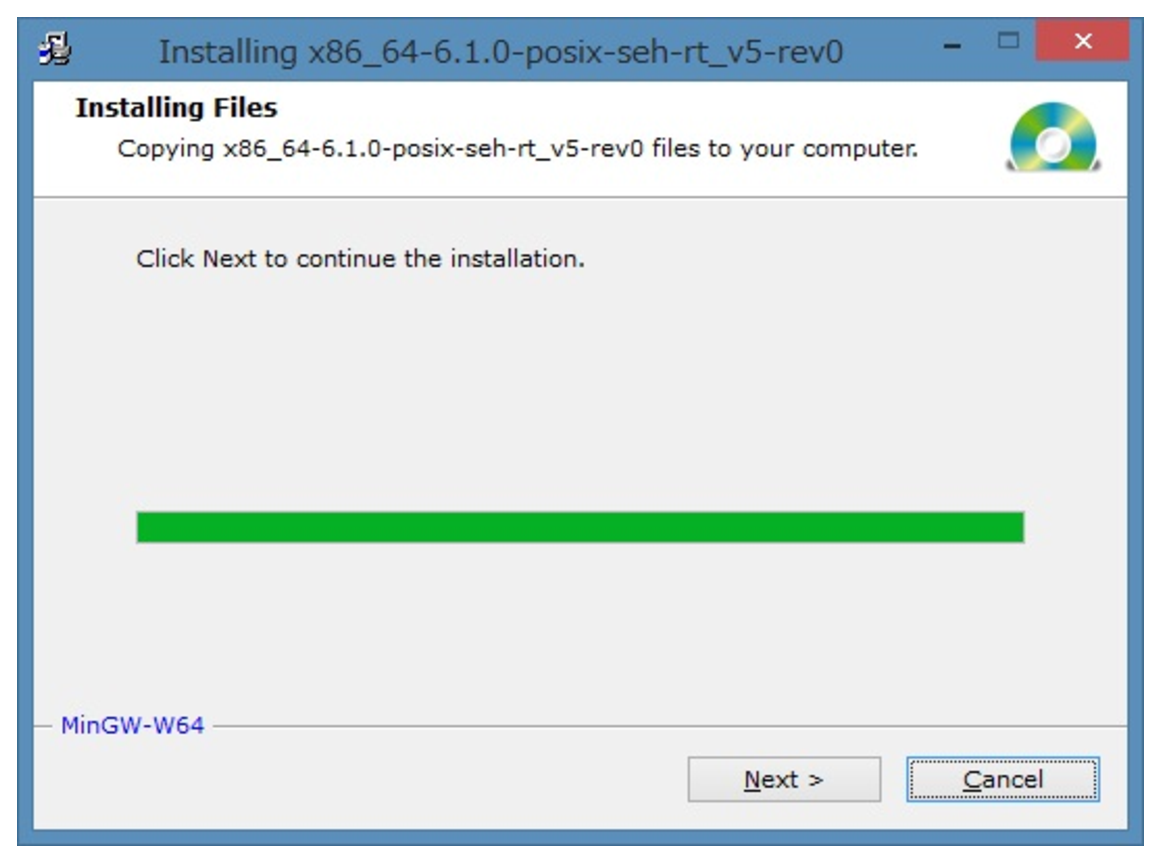
\includegraphics[width=0.45\linewidth]{appendix/install/1/install5.eps}} \hspace{5mm}
\subfloat[]{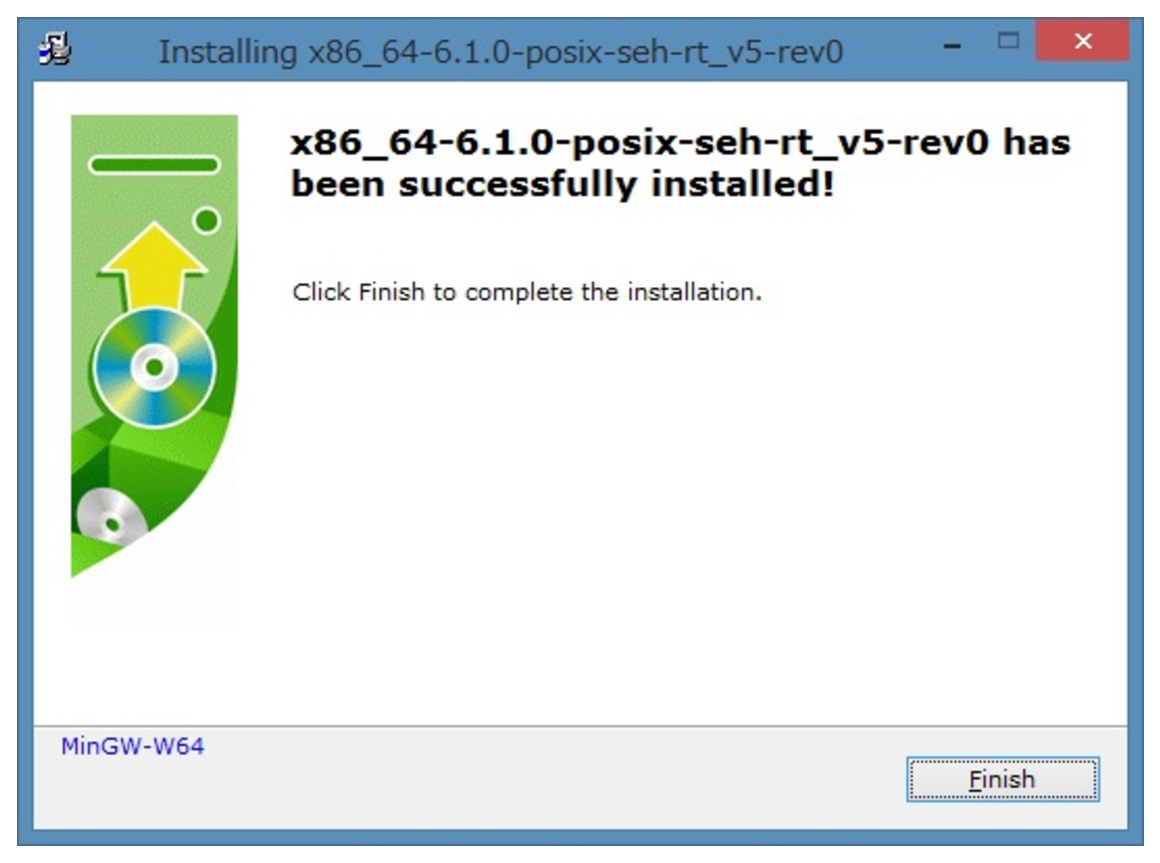
\includegraphics[width=0.45\linewidth]{appendix/install/1/install6.eps}}\\
\caption{gfotranのインストール.  }
\label{fig_install}
\end{figure}


\end{document}
